\pdfoutput=1
%% Author: PGL  Porta Mana
%% Created: 2015-05-01T20:53:34+0200
%% Last-Updated: 2024-01-18T12:14:17+0100
%%%%%%%%%%%%%%%%%%%%%%%%%%%%%%%%%%%%%%%%%%%%%%%%%%%%%%%%%%%%%%%%%%%%%%%%%%%%
\newif\ifarxiv
\arxivfalse
%\iftrue\pdfmapfile{+classico.map}\fi
\newif\ifafour
\afourfalse% true = A4, false = A5
\newif\iftypodisclaim % typographical disclaim on the side
\typodisclaimtrue
\newcommand*{\memfontfamily}{zplr}
\newcommand*{\memfontpack}{newpx}
\documentclass[\ifafour a4paper,12pt,\else a5paper,10pt,\fi%extrafontsizes,%
onecolumn,oneside,article,%french,italian,german,swedish,latin,
british%
]{memoir}
\newcommand*{\firstdraft}{26 May 2023}
\newcommand*{\firstpublished}{\firstdraft}
\newcommand*{\updated}{\ifarxiv***\else\today\fi}
\newcommand*{\propertitle}{Introduction to 21st-century physics}
\newcommand*{\pdftitle}{\propertitle}
\newcommand*{\headtitle}{21st-century physics (ING175)}
\newcommand*{\pdfauthor}{P.G.L.  Porta Mana}
\newcommand*{\headauthor}{Luca}
\newcommand*{\reporthead}{\iftrue\else Open Science Framework \href{https://doi.org/10.31219/osf.io/***}{\textsc{doi}:10.31219/osf.io/***}\fi}% Report number

%%%%%%%%%%%%%%%%%%%%%%%%%%%%%%%%%%%%%%%%%%%%%%%%%%%%%%%%%%%%%%%%%%%%%%%%%%%%
%%% Calls to packages (uncomment as needed)
%%%%%%%%%%%%%%%%%%%%%%%%%%%%%%%%%%%%%%%%%%%%%%%%%%%%%%%%%%%%%%%%%%%%%%%%%%%%

%\usepackage{pifont}

%\usepackage{fontawesome}
\PassOptionsToPackage{obeyspaces}{url}
\usepackage[T1]{fontenc}
\input{glyphtounicode} \pdfgentounicode=1

\usepackage[utf8]{inputenx}

%\usepackage{newunicodechar}
% \newunicodechar{Ĕ}{\u{E}}
% \newunicodechar{ĕ}{\u{e}}
% \newunicodechar{Ĭ}{\u{I}}
% \newunicodechar{ĭ}{\u{\i}}
% \newunicodechar{Ŏ}{\u{O}}
% \newunicodechar{ŏ}{\u{o}}
% \newunicodechar{Ŭ}{\u{U}}
% \newunicodechar{ŭ}{\u{u}}
% \newunicodechar{Ā}{\=A}
% \newunicodechar{ā}{\=a}
% \newunicodechar{Ē}{\=E}
% \newunicodechar{ē}{\=e}
% \newunicodechar{Ī}{\=I}
% \newunicodechar{ī}{\={\i}}
% \newunicodechar{Ō}{\=O}
% \newunicodechar{ō}{\=o}
% \newunicodechar{Ū}{\=U}
% \newunicodechar{ū}{\=u}
% \newunicodechar{Ȳ}{\=Y}
% \newunicodechar{ȳ}{\=y}

\newcommand*{\bmmax}{0} % reduce number of bold fonts, before font packages
\newcommand*{\hmmax}{0} % reduce number of heavy fonts, before font packages

\usepackage{textcomp}

%\usepackage[normalem]{ulem}% package for underlining
% \makeatletter
% \def\ssout{\bgroup \ULdepth=-.35ex%\UL@setULdepth
%  \markoverwith{\lower\ULdepth\hbox
%    {\kern-.03em\vbox{\hrule width.2em\kern1.2\p@\hrule}\kern-.03em}}%
%  \ULon}
% \makeatother

\usepackage{amsmath}

\usepackage{mathtools}
%\addtolength{\jot}{\jot} % increase spacing in multiline formulae
\setlength{\multlinegap}{0pt}

%\usepackage{empheq}% automatically calls amsmath and mathtools
%\newcommand*{\widefbox}[1]{\fbox{\hspace{1em}#1\hspace{1em}}}

%%%% empheq above seems more versatile than these:
%\usepackage{fancybox}
%\usepackage{framed}

% \usepackage[misc]{ifsym} % for dice
% \newcommand*{\diceone}{{\scriptsize\Cube{1}}}

\usepackage{amssymb}

\usepackage{amsxtra}

\usepackage[main=british]{babel}\selectlanguage{british}
%\newcommand*{\langnohyph}{\foreignlanguage{nohyphenation}}
\newcommand{\langnohyph}[1]{\begin{hyphenrules}{nohyphenation}#1\end{hyphenrules}}

\usepackage[autostyle=false,autopunct=false,english=british]{csquotes}
\setquotestyle{american}
\newcommand*{\defquote}[1]{`\,#1\,'}

% \makeatletter
% \renewenvironment{quotation}%
%                {\list{}{\listparindent 1.5em%
%                         \itemindent    \listparindent
%                         \rightmargin=1em   \leftmargin=1em
%                         \parsep        \z@ \@plus\p@}%
%                 \item[]\footnotesize}%
%                 {\endlist}
% \makeatother


\usepackage{amsthm}
%% from https://tex.stackexchange.com/a/404680/97039
\makeatletter
\def\@endtheorem{\endtrivlist}
\makeatother

\newcommand*{\QED}{\textsc{q.e.d.}}
\renewcommand*{\qedsymbol}{\QED}
\theoremstyle{remark}
\newtheorem{note}{Note}
\newtheorem*{remark}{Note}
\newtheoremstyle{innote}{\parsep}{\parsep}{\footnotesize}{}{}{}{0pt}{}
\theoremstyle{innote}
\newtheorem*{innote}{}

\usepackage[shortlabels,inline]{enumitem}
\SetEnumitemKey{para}{itemindent=\parindent,leftmargin=0pt,listparindent=\parindent,parsep=0pt,itemsep=\topsep}
% \begin{asparaenum} = \begin{enumerate}[para]
% \begin{inparaenum} = \begin{enumerate*}
\setlist{itemsep=0pt,topsep=\parsep}
\setlist[enumerate,2]{label=(\roman*)}
\setlist[enumerate]{label=(\alph*),leftmargin=1.5\parindent}
\setlist[itemize]{leftmargin=1.5\parindent}
\setlist[description]{leftmargin=1.5\parindent}
% old alternative:
% \setlist[enumerate,2]{label=\alph*.}
% \setlist[enumerate]{leftmargin=\parindent}
% \setlist[itemize]{leftmargin=\parindent}
% \setlist[description]{leftmargin=\parindent}

\usepackage[babel,theoremfont,largesc,smallerops,nosymbolsc]{newpx}

% For Baskerville see https://ctan.org/tex-archive/fonts/baskervillef?lang=en
% and http://mirrors.ctan.org/fonts/baskervillef/doc/baskervillef-doc.pdf
% \usepackage[p]{baskervillef}
% \usepackage[varqu,varl,var0]{inconsolata}
% \usepackage[scale=.95,type1]{cabin}
% \usepackage[baskerville,vvarbb]{newtxmath}
% \usepackage[cal=boondoxo]{mathalfa}


% \usepackage[bigdelims,nosymbolsc%,smallerops % probably arXiv doesn't have it
% ]{newpxmath}
%\useosf
%\linespread{1.083}%
%\linespread{1.05}% widely used
\linespread{1.1}% best for text with maths
%% smaller operators for old version of newpxmath
\makeatletter
\def\re@DeclareMathSymbol#1#2#3#4{%
    \let#1=\undefined
    \DeclareMathSymbol{#1}{#2}{#3}{#4}}
%\re@DeclareMathSymbol{\bigsqcupop}{\mathop}{largesymbols}{"46}
%\re@DeclareMathSymbol{\bigodotop}{\mathop}{largesymbols}{"4A}
\re@DeclareMathSymbol{\bigoplusop}{\mathop}{largesymbols}{"4C}
\re@DeclareMathSymbol{\bigotimesop}{\mathop}{largesymbols}{"4E}
\re@DeclareMathSymbol{\sumop}{\mathop}{largesymbols}{"50}
\re@DeclareMathSymbol{\prodop}{\mathop}{largesymbols}{"51}
\re@DeclareMathSymbol{\bigcupop}{\mathop}{largesymbols}{"53}
\re@DeclareMathSymbol{\bigcapop}{\mathop}{largesymbols}{"54}
%\re@DeclareMathSymbol{\biguplusop}{\mathop}{largesymbols}{"55}
\re@DeclareMathSymbol{\bigwedgeop}{\mathop}{largesymbols}{"56}
\re@DeclareMathSymbol{\bigveeop}{\mathop}{largesymbols}{"57}
%\re@DeclareMathSymbol{\bigcupdotop}{\mathop}{largesymbols}{"DF}
%\re@DeclareMathSymbol{\bigcapplusop}{\mathop}{largesymbolsPXA}{"00}
%\re@DeclareMathSymbol{\bigsqcupplusop}{\mathop}{largesymbolsPXA}{"02}
%\re@DeclareMathSymbol{\bigsqcapplusop}{\mathop}{largesymbolsPXA}{"04}
%\re@DeclareMathSymbol{\bigsqcapop}{\mathop}{largesymbolsPXA}{"06}
\re@DeclareMathSymbol{\bigtimesop}{\mathop}{largesymbolsPXA}{"10}
%\re@DeclareMathSymbol{\coprodop}{\mathop}{largesymbols}{"60}
%\re@DeclareMathSymbol{\varprod}{\mathop}{largesymbolsPXA}{16}
\makeatother
%%
%% With euler font cursive for Greek letters - the [1] means 100% scaling
\DeclareFontFamily{U}{egreek}{\skewchar\font'177}%
\DeclareFontShape{U}{egreek}{m}{n}{<-6>s*[1]eurm5 <6-8>s*[1]eurm7 <8->s*[1]eurm10}{}%
\DeclareFontShape{U}{egreek}{m}{it}{<->s*[1]eurmo10}{}%
\DeclareFontShape{U}{egreek}{b}{n}{<-6>s*[1]eurb5 <6-8>s*[1]eurb7 <8->s*[1]eurb10}{}%
\DeclareFontShape{U}{egreek}{b}{it}{<->s*[1]eurbo10}{}%
\DeclareSymbolFont{egreeki}{U}{egreek}{m}{it}%
\SetSymbolFont{egreeki}{bold}{U}{egreek}{b}{it}% from the amsfonts package
\DeclareSymbolFont{egreekr}{U}{egreek}{m}{n}%
\SetSymbolFont{egreekr}{bold}{U}{egreek}{b}{n}% from the amsfonts package
% Take also \sum, \prod, \coprod symbols from Euler fonts
\DeclareFontFamily{U}{egreekx}{\skewchar\font'177}
\DeclareFontShape{U}{egreekx}{m}{n}{%
       <-7.5>s*[0.9]euex7%
    <7.5-8.5>s*[0.9]euex8%
    <8.5-9.5>s*[0.9]euex9%
    <9.5->s*[0.9]euex10%
}{}
\DeclareSymbolFont{egreekx}{U}{egreekx}{m}{n}
\DeclareMathSymbol{\sumop}{\mathop}{egreekx}{"50}
\DeclareMathSymbol{\prodop}{\mathop}{egreekx}{"51}
\DeclareMathSymbol{\coprodop}{\mathop}{egreekx}{"60}
\makeatletter
\def\sum{\DOTSI\sumop\slimits@}
\def\prod{\DOTSI\prodop\slimits@}
\def\coprod{\DOTSI\coprodop\slimits@}
\makeatother
%%%% Greek letters not usually given in LaTeX
%%%% best to uncomment only the ones needed
%% %% \input{definegreek.tex} % originally in a separate file
\DeclareMathSymbol{\varpartial}{\mathalpha}{egreeki}{"40}
%\DeclareMathSymbol{\partialup}{\mathalpha}{egreekr}{"40}
% \DeclareMathSymbol{\alpha}{\mathalpha}{egreeki}{"0B}
% \DeclareMathSymbol{\beta}{\mathalpha}{egreeki}{"0C}
% \DeclareMathSymbol{\gamma}{\mathalpha}{egreeki}{"0D}
% \DeclareMathSymbol{\delta}{\mathalpha}{egreeki}{"0E}
% \DeclareMathSymbol{\epsilon}{\mathalpha}{egreeki}{"0F}
% \DeclareMathSymbol{\zeta}{\mathalpha}{egreeki}{"10}
% \DeclareMathSymbol{\eta}{\mathalpha}{egreeki}{"11}
% \DeclareMathSymbol{\theta}{\mathalpha}{egreeki}{"12}
% \DeclareMathSymbol{\iota}{\mathalpha}{egreeki}{"13}
% \DeclareMathSymbol{\kappa}{\mathalpha}{egreeki}{"14}
% \DeclareMathSymbol{\lambda}{\mathalpha}{egreeki}{"15}
% \DeclareMathSymbol{\mu}{\mathalpha}{egreeki}{"16}
% \DeclareMathSymbol{\nu}{\mathalpha}{egreeki}{"17}
% \DeclareMathSymbol{\xi}{\mathalpha}{egreeki}{"18}
% \DeclareMathSymbol{\omicron}{\mathalpha}{egreeki}{"6F}
% \DeclareMathSymbol{\pi}{\mathalpha}{egreeki}{"19}
% \DeclareMathSymbol{\rho}{\mathalpha}{egreeki}{"1A}
% \DeclareMathSymbol{\sigma}{\mathalpha}{egreeki}{"1B}
% \DeclareMathSymbol{\tau}{\mathalpha}{egreeki}{"1C}
% \DeclareMathSymbol{\upsilon}{\mathalpha}{egreeki}{"1D}
% \DeclareMathSymbol{\phi}{\mathalpha}{egreeki}{"1E}
% \DeclareMathSymbol{\chi}{\mathalpha}{egreeki}{"1F}
% \DeclareMathSymbol{\psi}{\mathalpha}{egreeki}{"20}
% \DeclareMathSymbol{\omega}{\mathalpha}{egreeki}{"21}
% \DeclareMathSymbol{\varepsilon}{\mathalpha}{egreeki}{"22}
% \DeclareMathSymbol{\vartheta}{\mathalpha}{egreeki}{"23}
% \DeclareMathSymbol{\varpi}{\mathalpha}{egreeki}{"24}
% \let\varrho\rho 
% \let\varsigma\sigma
% \let\varkappa\kappa
% \DeclareMathSymbol{\varphi}{\mathalpha}{egreeki}{"27}
% %
% \DeclareMathSymbol{\varAlpha}{\mathalpha}{egreeki}{"41}
% \DeclareMathSymbol{\varBeta}{\mathalpha}{egreeki}{"42}
% \DeclareMathSymbol{\varGamma}{\mathalpha}{egreeki}{"00}
% \DeclareMathSymbol{\varDelta}{\mathalpha}{egreeki}{"01}
% \DeclareMathSymbol{\varEpsilon}{\mathalpha}{egreeki}{"45}
% \DeclareMathSymbol{\varZeta}{\mathalpha}{egreeki}{"5A}
% \DeclareMathSymbol{\varEta}{\mathalpha}{egreeki}{"48}
% \DeclareMathSymbol{\varTheta}{\mathalpha}{egreeki}{"02}
% \DeclareMathSymbol{\varIota}{\mathalpha}{egreeki}{"49}
% \DeclareMathSymbol{\varKappa}{\mathalpha}{egreeki}{"4B}
% \DeclareMathSymbol{\varLambda}{\mathalpha}{egreeki}{"03}
% \DeclareMathSymbol{\varMu}{\mathalpha}{egreeki}{"4D}
% \DeclareMathSymbol{\varNu}{\mathalpha}{egreeki}{"4E}
% \DeclareMathSymbol{\varXi}{\mathalpha}{egreeki}{"04}
% \DeclareMathSymbol{\varOmicron}{\mathalpha}{egreeki}{"4F}
% \DeclareMathSymbol{\varPi}{\mathalpha}{egreeki}{"05}
% \DeclareMathSymbol{\varRho}{\mathalpha}{egreeki}{"50}
% \DeclareMathSymbol{\varSigma}{\mathalpha}{egreeki}{"06}
% \DeclareMathSymbol{\varTau}{\mathalpha}{egreeki}{"54}
% \DeclareMathSymbol{\varUpsilon}{\mathalpha}{egreeki}{"07}
% \DeclareMathSymbol{\varPhi}{\mathalpha}{egreeki}{"08}
% \DeclareMathSymbol{\varChi}{\mathalpha}{egreeki}{"58}
% \DeclareMathSymbol{\varPsi}{\mathalpha}{egreeki}{"09}
% \DeclareMathSymbol{\varOmega}{\mathalpha}{egreeki}{"0A} 
% %
% \DeclareMathSymbol{\Alpha}{\mathalpha}{egreekr}{"41}
% \DeclareMathSymbol{\Beta}{\mathalpha}{egreekr}{"42}
% \DeclareMathSymbol{\Gamma}{\mathalpha}{egreekr}{"00}
% \DeclareMathSymbol{\Delta}{\mathalpha}{egreekr}{"01}
% \DeclareMathSymbol{\Epsilon}{\mathalpha}{egreekr}{"45}
% \DeclareMathSymbol{\Zeta}{\mathalpha}{egreekr}{"5A}
% \DeclareMathSymbol{\Eta}{\mathalpha}{egreekr}{"48}
% \DeclareMathSymbol{\Theta}{\mathalpha}{egreekr}{"02}
% \DeclareMathSymbol{\Iota}{\mathalpha}{egreekr}{"49}
% \DeclareMathSymbol{\Kappa}{\mathalpha}{egreekr}{"4B}
% \DeclareMathSymbol{\Lambda}{\mathalpha}{egreekr}{"03}
% \DeclareMathSymbol{\Mu}{\mathalpha}{egreekr}{"4D}
% \DeclareMathSymbol{\Nu}{\mathalpha}{egreekr}{"4E}
% \DeclareMathSymbol{\Xi}{\mathalpha}{egreekr}{"04}
% \DeclareMathSymbol{\Omicron}{\mathalpha}{egreekr}{"4F}
% \DeclareMathSymbol{\Pi}{\mathalpha}{egreekr}{"05}
% \DeclareMathSymbol{\Rho}{\mathalpha}{egreekr}{"50}
% \DeclareMathSymbol{\Sigma}{\mathalpha}{egreekr}{"06}
% \DeclareMathSymbol{\Tau}{\mathalpha}{egreekr}{"54}
% \DeclareMathSymbol{\Upsilon}{\mathalpha}{egreekr}{"07}
% \DeclareMathSymbol{\Phi}{\mathalpha}{egreekr}{"08}
% \DeclareMathSymbol{\Chi}{\mathalpha}{egreekr}{"58}
% \DeclareMathSymbol{\Psi}{\mathalpha}{egreekr}{"09}
% \DeclareMathSymbol{\Omega}{\mathalpha}{egreekr}{"0A}
% %
% \DeclareMathSymbol{\alphaup}{\mathalpha}{egreekr}{"0B}
% \DeclareMathSymbol{\betaup}{\mathalpha}{egreekr}{"0C}
% \DeclareMathSymbol{\gammaup}{\mathalpha}{egreekr}{"0D}
\DeclareMathSymbol{\deltaup}{\mathalpha}{egreekr}{"0E}
% \DeclareMathSymbol{\epsilonup}{\mathalpha}{egreekr}{"0F}
% \DeclareMathSymbol{\zetaup}{\mathalpha}{egreekr}{"10}
% \DeclareMathSymbol{\etaup}{\mathalpha}{egreekr}{"11}
% \DeclareMathSymbol{\thetaup}{\mathalpha}{egreekr}{"12}
% \DeclareMathSymbol{\iotaup}{\mathalpha}{egreekr}{"13}
% \DeclareMathSymbol{\kappaup}{\mathalpha}{egreekr}{"14}
% \DeclareMathSymbol{\lambdaup}{\mathalpha}{egreekr}{"15}
% \DeclareMathSymbol{\muup}{\mathalpha}{egreekr}{"16}
% \DeclareMathSymbol{\nuup}{\mathalpha}{egreekr}{"17}
% \DeclareMathSymbol{\xiup}{\mathalpha}{egreekr}{"18}
% \DeclareMathSymbol{\omicronup}{\mathalpha}{egreekr}{"6F}
\DeclareMathSymbol{\piup}{\mathalpha}{egreekr}{"19}
% \DeclareMathSymbol{\rhoup}{\mathalpha}{egreekr}{"1A}
% \DeclareMathSymbol{\sigmaup}{\mathalpha}{egreekr}{"1B}
% \DeclareMathSymbol{\tauup}{\mathalpha}{egreekr}{"1C}
% \DeclareMathSymbol{\upsilonup}{\mathalpha}{egreekr}{"1D}
% \DeclareMathSymbol{\phiup}{\mathalpha}{egreekr}{"1E}
% \DeclareMathSymbol{\chiup}{\mathalpha}{egreekr}{"1F}
% \DeclareMathSymbol{\psiup}{\mathalpha}{egreekr}{"20}
% \DeclareMathSymbol{\omegaup}{\mathalpha}{egreekr}{"21}
% \DeclareMathSymbol{\varepsilonup}{\mathalpha}{egreekr}{"22}
% \DeclareMathSymbol{\varthetaup}{\mathalpha}{egreekr}{"23}
% \DeclareMathSymbol{\varpiup}{\mathalpha}{egreekr}{"24}
% \let\varrhoup\rhoup 
% \let\varsigmaup\sigmaup
% \let\varkappaup\kappaup
% \DeclareMathSymbol{\varphiup}{\mathalpha}{egreekr}{"27}


% \usepackage%[scaled=0.9]%
% {classico}%  Optima as sans-serif font
\renewcommand\sfdefault{uop}
\DeclareMathAlphabet{\mathsf}  {T1}{\sfdefault}{m}{sl}
\SetMathAlphabet{\mathsf}{bold}{T1}{\sfdefault}{b}{sl}
%\newcommand*{\mathte}[1]{\textbf{\textit{\textsf{#1}}}}
% Upright sans-serif math alphabet
% \DeclareMathAlphabet{\mathsu}  {T1}{\sfdefault}{m}{n}
% \SetMathAlphabet{\mathsu}{bold}{T1}{\sfdefault}{b}{n}

% DejaVu Mono as typewriter text
\usepackage[scaled=0.84]{DejaVuSansMono}

\usepackage{mathdots}

\usepackage[usenames]{xcolor}
% Tol (2012) colour-blind-, print-, screen-friendly colours, alternative scheme; Munsell terminology
\definecolor{bluepurple}{RGB}{68,119,170}
\definecolor{blue}{RGB}{102,204,238}
\definecolor{green}{RGB}{34,136,51}
\definecolor{yellow}{RGB}{204,187,68}
\definecolor{red}{RGB}{238,102,119}
\definecolor{redpurple}{RGB}{170,51,119}
\definecolor{grey}{RGB}{187,187,187}
% Tol (2012) colour-blind-, print-, screen-friendly colours; Munsell terminology
% \definecolor{lbpurple}{RGB}{51,34,136}
% \definecolor{lblue}{RGB}{136,204,238}
% \definecolor{lbgreen}{RGB}{68,170,153}
% \definecolor{lgreen}{RGB}{17,119,51}
% \definecolor{lgyellow}{RGB}{153,153,51}
% \definecolor{lyellow}{RGB}{221,204,119}
% \definecolor{lred}{RGB}{204,102,119}
% \definecolor{lpred}{RGB}{136,34,85}
% \definecolor{lrpurple}{RGB}{170,68,153}
\definecolor{lgrey}{RGB}{221,221,221}
%\newcommand*\mycolourbox[1]{%
%\colorbox{grey}{\hspace{1em}#1\hspace{1em}}}
\colorlet{shadecolor}{lgrey}

\usepackage{bm}

\usepackage{microtype}

\usepackage[backend=biber,mcite,%subentry,
citestyle=authoryear-comp,bibstyle=pglpm_latex/pglpm-authoryear,autopunct=false,sorting=ny,sortcites=false,natbib=false,maxcitenames=2,maxbibnames=8,minbibnames=8,giveninits=true,uniquename=false,uniquelist=false,maxalphanames=1,block=space,hyperref=true,defernumbers=false,useprefix=true,sortupper=false,language=british,parentracker=false,autocite=footnote]{biblatex}
\DeclareSortingTemplate{ny}{\sort{\field{sortname}\field{author}\field{editor}}\sort{\field{year}}}
\DeclareFieldFormat{postnote}{#1}
\iffalse\makeatletter%%% replace parenthesis with brackets
\newrobustcmd*{\parentexttrack}[1]{%
  \begingroup
  \blx@blxinit
  \blx@setsfcodes
  \blx@bibopenparen#1\blx@bibcloseparen
  \endgroup}
\AtEveryCite{%
  \let\parentext=\parentexttrack%
  \let\bibopenparen=\bibopenbracket%
  \let\bibcloseparen=\bibclosebracket}
\makeatother\fi
\DefineBibliographyExtras{british}{\def\finalandcomma{\addcomma}}
\renewcommand*{\finalnamedelim}{\addspace\amp\space}
% \renewcommand*{\finalnamedelim}{\addcomma\space}
\renewcommand*{\textcitedelim}{\addcomma\space}
% \setcounter{biburlnumpenalty}{1} % to allow url breaks anywhere
% \setcounter{biburlucpenalty}{0}
% \setcounter{biburllcpenalty}{1}
\setcounter{biburlucpenalty}{1}  %break URL after uppercase character
\setcounter{biburlnumpenalty}{1} %break URL after number
\setcounter{biburllcpenalty}{1}  %break URL after lowercase character
\DeclareDelimFormat{multicitedelim}{\addsemicolon\addspace\space}
\DeclareDelimFormat{compcitedelim}{\addsemicolon\addspace\space}
\DeclareDelimFormat{postnotedelim}{\addspace}
\ifarxiv\else\addbibresource{portamanabib.bib}\fi
\renewcommand{\bibfont}{\footnotesize}
%\appto{\citesetup}{\footnotesize}% smaller font for citations
\defbibheading{bibliography}[\bibname]{\section*{#1}\addcontentsline{toc}{section}{#1}%\markboth{#1}{#1}
}
\newcommand*{\citep}{\footcites}
\newcommand*{\citey}{\footcites}%{\parencites*}
\newcommand*{\ibid}{\unspace\addtocounter{footnote}{-1}\footnotemark{}}
%\renewcommand*{\cite}{\parencite}
%\renewcommand*{\cites}{\parencites}
\providecommand{\href}[2]{#2}
\providecommand{\eprint}[2]{\texttt{\href{#1}{#2}}}
\newcommand*{\amp}{\&}
% \newcommand*{\citein}[2][]{\textnormal{\textcite[#1]{#2}}%\addtocategory{extras}{#2}
% }
\newcommand*{\citein}[2][]{\textnormal{\textcite[#1]{#2}}%\addtocategory{extras}{#2}
}
\newcommand*{\citebi}[2][]{\textcite[#1]{#2}%\addtocategory{extras}{#2}
}
\newcommand*{\subtitleproc}[1]{}
\newcommand*{\chapb}{ch.}
%
%\def\UrlOrds{\do\*\do\-\do\~\do\'\do\"\do\-}%
% \def\myUrlOrds{\do\0\do\1\do\2\do\3\do\4\do\5\do\6\do\7\do\8\do\9\do\a\do\b\do\c\do\d\do\e\do\f\do\g\do\h\do\i\do\j\do\k\do\l\do\m\do\n\do\o\do\p\do\q\do\r\do\s\do\t\do\u\do\v\do\w\do\x\do\y\do\z\do\A\do\B\do\C\do\D\do\E\do\F\do\G\do\H\do\I\do\J\do\K\do\L\do\M\do\N\do\O\do\P\do\Q\do\R\do\S\do\T\do\U\do\V\do\W\do\X\do\Y\do\Z}%
\makeatletter
%\g@addto@macro\UrlSpecials{\do={\newline}}
\g@addto@macro{\UrlBreaks}{%
\do\0\do\1\do\2\do\3\do\4\do\5\do\6\do\7\do\8\do\9\do\a\do\b\do\c\do\d\do\e\do\f\do\g\do\h\do\i\do\j\do\k\do\l\do\m\do\n\do\o\do\p\do\q\do\r\do\s\do\t\do\u\do\v\do\w\do\x\do\y\do\z\do\A\do\B\do\C\do\D\do\E\do\F\do\G\do\H\do\I\do\J\do\K\do\L\do\M\do\N\do\O\do\P\do\Q\do\R\do\S\do\T\do\U\do\V\do\W\do\X\do\Y\do\Z%
}
% \g@addto@macro\UrlSpecials{%
% \do\/{\mbox{\UrlFont/}\hskip 0pt plus 10pt}%
% }
\makeatother
\newcommand*{\arxiveprint}[1]{%
arXiv \doi{10.48550/arXiv.#1}%
}
\newcommand*{\mparceprint}[1]{%
\href{http://www.ma.utexas.edu/mp_arc-bin/mpa?yn=#1}{mp_arc:\allowbreak\nolinkurl{#1}}%
}
\newcommand*{\haleprint}[1]{%
\href{https://hal.archives-ouvertes.fr/#1}{\textsc{hal}:\allowbreak\nolinkurl{#1}}%
}
\newcommand*{\philscieprint}[1]{%
\href{http://philsci-archive.pitt.edu/archive/#1}{PhilSci:\allowbreak\nolinkurl{#1}}%
}
\newcommand*{\doi}[1]{%
\href{https://doi.org/#1}{\textsc{doi}:\allowbreak\nolinkurl{#1}}%
}
\newcommand*{\biorxiveprint}[1]{%
bioRxiv \doi{10.1101/#1}%
}
\newcommand*{\osfeprint}[1]{%
Open Science Framework \doi{10.31219/osf.io/#1}%
}
\newcommand*{\osfproj}[1]{%
Open Science Framework \doi{10.17605/osf.io/#1}%
}

\usepackage{graphicx}

\usepackage{wrapfig2}

%\usepackage{tikz-cd}

\PassOptionsToPackage{hyphens}{url}\usepackage[hypertexnames=false,pdfencoding=unicode,psdextra]{hyperref}

\usepackage[depth=4]{bookmark}
\hypersetup{colorlinks=true,bookmarksnumbered,pdfborder={0 0 0.25},citebordercolor={0.2667 0.4667 0.6667},citecolor=bluepurple,linkbordercolor={0.6667 0.2 0.4667},linkcolor=redpurple,urlbordercolor={0.1333 0.5333 0.2},urlcolor=green,breaklinks=true,pdftitle={\pdftitle},pdfauthor={\pdfauthor}}
% \usepackage[vertfit=local]{breakurl}% only for arXiv
\providecommand*{\urlalt}{\href}

\usepackage{tensor}

\usepackage[british]{datetime2}
\DTMnewdatestyle{mydate}%
{% definitions
\renewcommand*{\DTMdisplaydate}[4]{%
\number##3\ \DTMenglishmonthname{##2} ##1}%
\renewcommand*{\DTMDisplaydate}{\DTMdisplaydate}%
}
\DTMsetdatestyle{mydate}

%%%%%%%%%%%%%%%%%%%%%%%%%%%%%%%%%%%%%%%%%%%%%%%%%%%%%%%%%%%%%%%%%%%%%%%%%%%%
%%% Layout. I do not know on which kind of paper the reader will print the
%%% paper on (A4? letter? one-sided? double-sided?). So I choose A5, which
%%% provides a good layout for reading on screen and save paper if printed
%%% two pages per sheet. Average length line is 66 characters and page
%%% numbers are centred.
%%%%%%%%%%%%%%%%%%%%%%%%%%%%%%%%%%%%%%%%%%%%%%%%%%%%%%%%%%%%%%%%%%%%%%%%%%%%
\ifafour\setstocksize{297mm}{210mm}%{*}% A4
\else\setstocksize{210mm}{5.5in}%{*}% 210x139.7
\fi
\settrimmedsize{\stockheight}{\stockwidth}{*}
\setlxvchars[\normalfont] %313.3632pt for a 66-characters line
\setxlvchars[\normalfont]
% \setlength{\trimtop}{0pt}
% \setlength{\trimedge}{\stockwidth}
% \addtolength{\trimedge}{-\paperwidth}
%\settrims{0pt}{0pt}
% The length of the normalsize alphabet is 133.05988pt - 10 pt = 26.1408pc
% The length of the normalsize alphabet is 159.6719pt - 12pt = 30.3586pc
% Bringhurst gives 32pc as boundary optimal with 69 ch per line
% The length of the normalsize alphabet is 191.60612pt - 14pt = 35.8634pc
\ifafour\settypeblocksize{*}{32pc}{1.618} % A4
%\setulmargins{*}{*}{1.667}%gives 5/3 margins % 2 or 1.667
\else\settypeblocksize{*}{26pc}{1.618}% nearer to a 66-line newpx and preserves GR
\fi
\setulmargins{*}{*}{1}%gives equal margins
\setlrmargins{*}{*}{*}
\setheadfoot{\onelineskip}{2.5\onelineskip}
\setheaderspaces{*}{2\onelineskip}{*}
\setmarginnotes{2ex}{10mm}{0pt}
\checkandfixthelayout[nearest]
%%% End layout
%% this fixes missing white spaces
%\pdfmapline{+dummy-space <dummy-space.pfb}
%\pdfinterwordspaceon% seems to add a white margin to Sumatrapdf

%%% Sectioning
\newcommand*{\asudedication}[1]{%
{\par\centering\textit{#1}\par}}
\newenvironment{acknowledgements}{\section*{Thanks}\addcontentsline{toc}{section}{Thanks}}{\par}
\makeatletter\renewcommand{\appendix}{\par
  \bigskip{\centering
   \interlinepenalty \@M
   \normalfont
   \printchaptertitle{\sffamily\appendixpagename}\par}
  \setcounter{section}{0}%
  \gdef\@chapapp{\appendixname}%
  \gdef\thesection{\@Alph\c@section}%
  \anappendixtrue}\makeatother
\counterwithout{section}{chapter}
\setsecnumformat{\upshape\csname the#1\endcsname\quad}
\setsecheadstyle{\large\bfseries\sffamily%
\centering}
\setsubsecheadstyle{\bfseries\sffamily%
\raggedright}
%\setbeforesecskip{-1.5ex plus 1ex minus .2ex}% plus 1ex minus .2ex}
%\setaftersecskip{1.3ex plus .2ex }% plus 1ex minus .2ex}
%\setsubsubsecheadstyle{\bfseries\sffamily\slshape\raggedright}
%\setbeforesubsecskip{1.25ex plus 1ex minus .2ex }% plus 1ex minus .2ex}
%\setaftersubsecskip{-1em}%{-0.5ex plus .2ex}% plus 1ex minus .2ex}
\setsubsecindent{0pt}%0ex plus 1ex minus .2ex}
\setparaheadstyle{\bfseries\sffamily%
\raggedright}
\setcounter{secnumdepth}{2}
\setlength{\headwidth}{\textwidth}
\newcommand{\addchap}[1]{\chapter*[#1]{#1}\addcontentsline{toc}{chapter}{#1}}
\newcommand{\addsec}[1]{\section*{#1}\addcontentsline{toc}{section}{#1}}
\newcommand{\addsubsec}[1]{\subsection*{#1}\addcontentsline{toc}{subsection}{#1}}
\newcommand{\addpara}[1]{\paragraph*{#1.}\addcontentsline{toc}{subsubsection}{#1}}
\newcommand{\addparap}[1]{\paragraph*{#1}\addcontentsline{toc}{subsubsection}{#1}}

%%% Headers, footers, pagestyle
\copypagestyle{manaart}{plain}
\makeheadrule{manaart}{\headwidth}{0.5\normalrulethickness}
\makeoddhead{manaart}{%
{\footnotesize%\sffamily%
\scshape\headauthor}}{}{{\footnotesize\sffamily%
\headtitle}}
\makeoddfoot{manaart}{}{\thepage}{}
\newcommand*\autanet{
\includegraphics[height=\heightof{M}]{autanet.pdf}}
\definecolor{mygray}{gray}{0.333}
\iftypodisclaim%
\ifafour\newcommand\addprintnote{\begin{picture}(0,0)%
\put(245,149){\makebox(0,0){\rotatebox{90}{\tiny\color{mygray}\textsf{This
            document is designed for screen reading and
            two-up printing on A4 or Letter paper}}}}%
\end{picture}}% A4
\else\newcommand\addprintnote{\begin{picture}(0,0)%
\put(176,112){\makebox(0,0){\rotatebox{90}{\tiny\color{mygray}\textsf{This
            document is designed for screen reading and
            two-up printing on A4 or Letter paper}}}}%
\end{picture}}\fi%afourtrue
\makeoddfoot{plain}{}{\makebox[0pt]{\thepage}\addprintnote}{}
\else
\makeoddfoot{plain}{}{\makebox[0pt]{\thepage}}{}
\fi%typodisclaimtrue
\makeoddhead{plain}{\scriptsize\reporthead}{}{}
% \copypagestyle{manainitial}{plain}
% \makeheadrule{manainitial}{\headwidth}{0.5\normalrulethickness}
% \makeoddhead{manainitial}{%
% \footnotesize\sffamily%
% \scshape\headauthor}{}{\footnotesize\sffamily%
% \headtitle}
% \makeoddfoot{manaart}{}{\thepage}{}

\pagestyle{manaart}

\setlength{\droptitle}{-3.9\onelineskip}
\pretitle{\begin{center}\LARGE\sffamily%
\bfseries}
\posttitle{\bigskip\end{center}}

\makeatletter\newcommand*{\atf}{
\includegraphics[totalheight=\heightof{@}]{pglpm_latex/atblack.png}}\makeatother
\providecommand{\affiliation}[1]{\textsl{\textsf{\footnotesize #1}}}
\providecommand{\epost}[1]{\texttt{\footnotesize\textless#1\textgreater}}
\providecommand{\email}[2]{\href{mailto:#1ZZ@#2 ((remove ZZ))}{#1\protect\atf#2}}
%\providecommand{\email}[2]{\href{mailto:#1@#2}{#1@#2}}

\preauthor{\vspace{-0.5\baselineskip}\begin{center}
\normalsize\sffamily%
\lineskip  0.5em}
\postauthor{\par\end{center}}
\predate{\DTMsetdatestyle{mydate}\begin{center}\footnotesize}
\postdate{\end{center}\vspace{-\medskipamount}}

\setfloatadjustment{figure}{\footnotesize}
\captiondelim{\quad}
\captionnamefont{\footnotesize\sffamily%
}
\captiontitlefont{\footnotesize}
%\firmlists*
\midsloppy
% handling orphan/widow lines, memman.pdf
% \clubpenalty=10000
% \widowpenalty=10000
% \raggedbottom
% Downes, memman.pdf
\clubpenalty=9996
\widowpenalty=9999
\brokenpenalty=4991
\predisplaypenalty=10000
\postdisplaypenalty=1549
\displaywidowpenalty=1602
\raggedbottom

\paragraphfootnotes
\setlength{\footmarkwidth}{2ex}
% \threecolumnfootnotes
%\setlength{\footmarksep}{0em}
\footmarkstyle{\textsuperscript{%\color{red}
\scriptsize\bfseries#1}~}
%\footmarkstyle{\textsuperscript{\color{red}\scriptsize\bfseries#1}~}
%\footmarkstyle{\textsuperscript{[#1]}~}

\selectlanguage{british}\frenchspacing

\definecolor{notecolour}{RGB}{68,170,153}
%\newcommand*{\puzzle}{\maltese}
\newcommand*{\puzzle}{{\fontencoding{U}\fontfamily{fontawesometwo}\selectfont\symbol{225}}}
\newcommand*{\wrench}{{\fontencoding{U}\fontfamily{fontawesomethree}\selectfont\symbol{114}}}
\newcommand*{\pencil}{{\fontencoding{U}\fontfamily{fontawesometwo}\selectfont\symbol{210}}}
\newcommand{\mynotew}[1]{{\footnotesize\color{notecolour}\wrench\ #1}}
\newcommand{\mynotep}[1]{{\footnotesize\color{notecolour}\pencil\ #1}}
\newcommand{\mynotez}[1]{{\footnotesize\color{notecolour}\puzzle\ #1}}

%%%%%%%%%%%%%%%%%%%%%%%%%%%%%%%%%%%%%%%%%%%%%%%%%%%%%%%%%%%%%%%%%%%%%%%%%%%%
%%% Paper's details
%%%%%%%%%%%%%%%%%%%%%%%%%%%%%%%%%%%%%%%%%%%%%%%%%%%%%%%%%%%%%%%%%%%%%%%%%%%%
\title{\propertitle}
\author{%
\hspace*{\stretch{1}}%
%% uncomment if additional authors present
% \parbox{0.5\linewidth}%\makebox[0pt][c]%
% {\protect\centering ***\\%
% \footnotesize\epost{\email{***}{***}}}%
% \hspace*{\stretch{1}}%
\parbox{1\linewidth}%\makebox[0pt][c]%
{\protect\centering Luca %P.G.L.  Porta Mana
 \href{https://orcid.org/0000-0002-6070-0784}{\protect
\includegraphics[scale=0.16]{pglpm_latex/orcid_32x32.png}}%
% \\\footnotesize
% Western Norway University of Applied Sciences%
% \quad\epost{\email{pgl}{portamana.org}}%
}%
%% uncomment if additional authors present
% \hspace*{\stretch{1}}%
% \parbox{0.5\linewidth}%\makebox[0pt][c]%
% {\protect\centering ***\\%
% \footnotesize\epost{\email{***}{***}}}%
\hspace*{\stretch{1}}%
}

%\date{Draft of \today\ (first drafted \firstdraft)}
\date{\firstpublished; updated \updated}

%%%%%%%%%%%%%%%%%%%%%%%%%%%%%%%%%%%%%%%%%%%%%%%%%%%%%%%%%%%%%%%%%%%%%%%%%%%%
%%% Macros @@@
%%%%%%%%%%%%%%%%%%%%%%%%%%%%%%%%%%%%%%%%%%%%%%%%%%%%%%%%%%%%%%%%%%%%%%%%%%%%

% Common ones - uncomment as needed
%\providecommand{\nequiv}{\not\equiv}
%\providecommand{\coloneqq}{\mathrel{\mathop:}=}
%\providecommand{\eqqcolon}{=\mathrel{\mathop:}}
%\providecommand{\varprod}{\prod}
\newcommand*{\de}{\uppartial}%partial diff
\newcommand*{\pu}{\piup}%constant pi
\newcommand*{\delt}{\deltaup}%Kronecker, Dirac
%\newcommand*{\eps}{\varepsilonup}%Levi-Civita, Heaviside
%\newcommand*{\riem}{\zetaup}%Riemann zeta
%\providecommand{\degree}{\textdegree}% degree
%\newcommand*{\celsius}{\textcelsius}% degree Celsius
%\newcommand*{\micro}{\textmu}% degree Celsius
% \newcommand*{\I}{\mathrm{i}}%imaginary unit
\newcommand*{\I}{\ensuremath{\mathrm{i}}}
% \newcommand*{\e}{\mathrm{e}}%Neper
\newcommand*{\e}{\ensuremath{\mathrm{e}}}
\newcommand*{\di}{\mathrm{d}}%differential
% \newcommand*{\dii}{\ensuremath{\mathrm{d}}}
% %% From TUGboat 18 (1997) 1 - leads to very strange spacing
% \makeatletter
% \providecommand*{\di}%
% {\@ifnextchar^{\DIfF}{\DIfF^{}}}
% \def\DIfF^#1{%
% \mathop{\mathrm{\mathstrut d}}%
% \nolimits^{#1}\gobblespace}
% \def\gobblespace{%
% \futurelet\diffarg\opspace}
% \def\opspace{%
% \let\DiffSpace\!%
% \ifx\diffarg(%
% \let\DiffSpace\relax
% \else
% \ifx\diffarg[%
% \let\DiffSpace\relax
% \else
% \ifx\diffarg\{%
% \let\DiffSpace\relax
% \fi\fi\fi\DiffSpace}
% \makeatother

% \newcommand*{\Di}{\mathrm{D}}%capital differential
%\newcommand*{\Li}{\mathrm{L}}%Lie derivative
%\newcommand*{\planckc}{\hslash}
%\newcommand*{\avogn}{N_{\textrm{A}}}
%\newcommand*{\NN}{\bm{\mathrm{N}}}
%\newcommand*{\ZZ}{\bm{\mathrm{Z}}}
%\newcommand*{\QQ}{\bm{\mathrm{Q}}}
\newcommand*{\RR}{\bm{\mathrm{R}}}
%\newcommand*{\CC}{\bm{\mathrm{C}}}
%\newcommand*{\nabl}{\bm{\nabla}}%nabla
%\DeclareMathOperator{\lb}{lb}%base 2 log
%\DeclareMathOperator{\tr}{tr}%trace
%\DeclareMathOperator{\card}{card}%cardinality
%% From TUGboat 18 (1997) 1
% \renewoperator{\Re}{\mathrm{Re}}{\nolimits}
% \renewoperator{\Im}{\mathrm{Im}}{\nolimits}
\DeclareMathOperator{\im}{Im}%im part
\DeclareMathOperator{\re}{Re}%re part
%\DeclareMathOperator{\sgn}{sgn}%signum
%\DeclareMathOperator{\ent}{ent}%integer less or equal to
%\DeclareMathOperator{\Ord}{O}%same order as
%\DeclareMathOperator{\ord}{o}%lower order than
%\newcommand*{\incr}{\triangle}%finite increment
\newcommand*{\defd}{\coloneqq}
\newcommand*{\defs}{\eqqcolon}
%\newcommand*{\Land}{\bigwedge}
%\newcommand*{\Lor}{\bigvee}
%\newcommand*{\lland}{\DOTSB\;\land\;}
%\newcommand*{\llor}{\DOTSB\;\lor\;}
\newcommand*{\limplies}{\mathbin{\Rightarrow}}%implies
%\newcommand*{\suchthat}{\mid}%{\mathpunct{|}}%such that (eg in sets)
%\newcommand*{\with}{\colon}%with (list of indices)
%\newcommand*{\mul}{\times}%multiplication
%\newcommand*{\inn}{\cdot}%inner product
%\newcommand*{\dotv}{\mathord{\,\cdot\,}}%variable place
%\newcommand*{\comp}{\circ}%composition of functions
%\newcommand*{\con}{\mathbin{:}}%scal prod of tensors
%\newcommand*{\equi}{\sim}%equivalent to 
\renewcommand*{\asymp}{\simeq}%equivalent to 
%\newcommand*{\corr}{\mathrel{\hat{=}}}%corresponds to
%\providecommand{\varparallel}{\ensuremath{\mathbin{/\mkern-7mu/}}}%parallel (tentative symbol)
\renewcommand*{\le}{\leqslant}%less or equal
\renewcommand*{\ge}{\geqslant}%greater or equal
%\DeclarePairedDelimiter\clcl{[}{]}
%\DeclarePairedDelimiter\clop{[}{[}
%\DeclarePairedDelimiter\opcl{]}{]}
%\DeclarePairedDelimiter\opop{]}{[}%}
\DeclarePairedDelimiter\abs{\lvert}{\rvert}
%\DeclarePairedDelimiter\norm{\lVert}{\rVert}
\DeclarePairedDelimiter\set{\{}{\}} %}
%\DeclareMathOperator{\pr}{P}%probability
\newcommand*{\p}{\mathrm{p}}%probability
\renewcommand*{\P}{\mathrm{P}}%probability
%\newcommand*{\E}{\mathrm{E}}
%% The "\:" space is chosen to correctly separate inner binary and external rels
\renewcommand*{\|}[1][]{\nonscript\:#1\vert\nonscript\:\mathopen{}}
%\DeclarePairedDelimiterX{\cp}[2]{(}{)}{#1\nonscript\:\delimsize\vert\nonscript\:\mathopen{}#2}
%\DeclarePairedDelimiterX{\ct}[2]{[}{]}{#1\nonscript\;\delimsize\vert\nonscript\:\mathopen{}#2}
%\DeclarePairedDelimiterX{\cs}[2]{\{}{\}}{#1\nonscript\:\delimsize\vert\nonscript\:\mathopen{}#2}
%\newcommand*{\+}{\lor}
%\renewcommand{\*}{\land}
%% symbol = for equality statements within probabilities
%% from https://tex.stackexchange.com/a/484142/97039
% \newcommand*{\eq}{\mathrel{\!=\!}}
% \let\texteq\=
% \renewcommand*{\=}{\TextOrMath\texteq\eq}
% \newcommand*{\eq}[1][=]{\mathrel{\!#1\!}}
\newcommand*{\mo}[1][=]{\mathclose{}\mathord{\nonscript\mkern0.5mu#1\nonscript\mkern0.5mu}\mathopen{}}
%%
\newcommand*{\sect}{\S}% Sect.~
\newcommand*{\sects}{\S\S}% Sect.~
\newcommand*{\chap}{ch.}%
\newcommand*{\chaps}{chs}%
\newcommand*{\bref}{ref.}%
\newcommand*{\brefs}{refs}%
%\newcommand*{\fn}{fn}%
\newcommand*{\eqn}{eq.}%
\newcommand*{\eqns}{eqs}%
\newcommand*{\fig}{fig.}%
\newcommand*{\figs}{figs}%
\newcommand*{\vs}{{vs}}
\newcommand*{\eg}{{e.g.}}
\newcommand*{\etc}{{etc.}}
\newcommand*{\ie}{{i.e.}}
%\newcommand*{\ca}{{c.}}
\newcommand*{\foll}{{ff.}}
%\newcommand*{\viz}{{viz}}
\newcommand*{\cf}{{cf.}}
%\newcommand*{\Cf}{{Cf.}}
%\newcommand*{\vd}{{v.}}
\newcommand*{\etal}{{et al.}}
%\newcommand*{\etsim}{{et sim.}}
%\newcommand*{\ibid}{{ibid.}}
%\newcommand*{\sic}{{sic}}
%\newcommand*{\id}{\mathte{I}}%id matrix
%\newcommand*{\nbd}{\nobreakdash}%
%\newcommand*{\bd}{\hspace{0pt}}%
%\def\hy{-\penalty0\hskip0pt\relax}
%\newcommand*{\labelbis}[1]{\tag*{(\ref{#1})$_\text{r}$}}
%\newcommand*{\mathbox}[2][.8]{\parbox[t]{#1\columnwidth}{#2}}
\newcommand*{\zerob}[1]{\makebox[0pt][l]{#1}}
\newcommand*{\tprod}{\mathop{\textstyle\prod}\nolimits}
\newcommand*{\tsum}{\mathop{\textstyle\sum}\nolimits}
%\newcommand*{\tint}{\begingroup\textstyle\int\endgroup\nolimits}
%\newcommand*{\tland}{\mathop{\textstyle\bigwedge}\nolimits}
%\newcommand*{\tlor}{\mathop{\textstyle\bigvee}\nolimits}
%\newcommand*{\sprod}{\mathop{\textstyle\prod}}
%\newcommand*{\ssum}{\mathop{\textstyle\sum}}
%\newcommand*{\sint}{\begingroup\textstyle\int\endgroup}
%\newcommand*{\sland}{\mathop{\textstyle\bigwedge}}
%\newcommand*{\slor}{\mathop{\textstyle\bigvee}}
%\newcommand*{\T}{^\transp}%transpose
%%\newcommand*{\QEM}%{\textnormal{$\Box$}}%{\ding{167}}
%\newcommand*{\qem}{\leavevmode\unskip\penalty9999 \hbox{}\nobreak\hfill
%\quad\hbox{\QEM}}
%% from TUGboat 18 (1997) 1:
%\providecommand*{\unit}[1]{\ensuremath{\mathrm{\,#1}}}

%%%%%%%%%%%%%%%%%%%%%%%%%%%%%%%%%%%%%%%%%%%%%%%%%%%%%%%%%%%%%%%%%%%%%%%%%%%%
%%% Custom macros for this file @@@
%%%%%%%%%%%%%%%%%%%%%%%%%%%%%%%%%%%%%%%%%%%%%%%%%%%%%%%%%%%%%%%%%%%%%%%%%%%%

\newcommand*{\widebar}[1]{{\mkern1.5mu\skew{2}\overline{\mkern-1.5mu#1\mkern-1.5mu}\mkern 1.5mu}}

% \newcommand{\explanation}[4][t]{%\setlength{\tabcolsep}{-1ex}
% %\smash{
% \begin{tabular}[#1]{c}#2\\[0.5\jot]\rule{1pt}{#3}\\#4\end{tabular}}%}
% \newcommand*{\ptext}[1]{\text{\small #1}}% for propositions
%\DeclareMathOperator*{\argsup}{arg\,sup}
\newcommand*{\dob}{degree of belief}
\newcommand*{\dobs}{degrees of belief}
\newcommand*{\yr}{\bm{r}}
%%% Custom macros end @@@

\usepackage{siunitx}
\usepackage{multimedia}

%%%%%%%%%%%%%%%%%%%%%%%%%%%%%%%%%%%%%%%%%%%%%%%%%%%%%%%%%%%%%%%%%%%%%%%%%%%%
%%% Beginning of document
%%%%%%%%%%%%%%%%%%%%%%%%%%%%%%%%%%%%%%%%%%%%%%%%%%%%%%%%%%%%%%%%%%%%%%%%%%%%
%\firmlists
\begin{document}
\captiondelim{\quad}\captionnamefont{\footnotesize}\captiontitlefont{\footnotesize}
\selectlanguage{british}\frenchspacing
\maketitle

%%%%%%%%%%%%%%%%%%%%%%%%%%%%%%%%%%%%%%%%%%%%%%%%%%%%%%%%%%%%%%%%%%%%%%%%%%%%
%%% Abstract
%%%%%%%%%%%%%%%%%%%%%%%%%%%%%%%%%%%%%%%%%%%%%%%%%%%%%%%%%%%%%%%%%%%%%%%%%%%%
\abstractrunin
\abslabeldelim{}
\renewcommand*{\abstractname}{}
\setlength{\absleftindent}{0pt}
\setlength{\absrightindent}{0pt}
\setlength{\abstitleskip}{-\absparindent}
\begin{abstract}\labelsep 0pt%
  \noindent Lecture notes on introductory mechanics and thermodynamics (ING175)
% \\\noindent\emph{\footnotesize Note: Dear Reader
%     \amp\ Peer, this manuscript is being peer-reviewed by you. Thank you.}
% \par%\\[\jot]
% \noindent
% {\footnotesize PACS: ***}\qquad%
% {\footnotesize MSC: ***}%
%\qquad{\footnotesize Keywords: ***}
\end{abstract}
\selectlanguage{british}\frenchspacing

%%%%%%%%%%%%%%%%%%%%%%%%%%%%%%%%%%%%%%%%%%%%%%%%%%%%%%%%%%%%%%%%%%%%%%%%%%%%
%%% Epigraph
%%%%%%%%%%%%%%%%%%%%%%%%%%%%%%%%%%%%%%%%%%%%%%%%%%%%%%%%%%%%%%%%%%%%%%%%%%%%
% \asudedication{\small ***}
% \vspace{\bigskipamount}
% \setlength{\epigraphwidth}{.7\columnwidth}
% %\epigraphposition{flushright}
% \epigraphtextposition{flushright}
% %\epigraphsourceposition{flushright}
% \epigraphfontsize{\footnotesize}
% \setlength{\epigraphrule}{0pt}
% %\setlength{\beforeepigraphskip}{0pt}
% %\setlength{\afterepigraphskip}{0pt}
% \epigraph{\emph{text}}{source}



%%%%%%%%%%%%%%%%%%%%%%%%%%%%%%%%%%%%%%%%%%%%%%%%%%%%%%%%%%%%%%%%%%%%%%%%%%%%
%%% BEGINNING OF MAIN TEXT
%%%%%%%%%%%%%%%%%%%%%%%%%%%%%%%%%%%%%%%%%%%%%%%%%%%%%%%%%%%%%%%%%%%%%%%%%%%%

\newpage
\setcounter{section}{-1}
\section{Introduction}
\label{sec:intro}

% \epigraphtextposition{flushright}
% %\epigraphsourceposition{flushright}
\epigraphfontsize{\footnotesize}
\setlength{\epigraphrule}{0pt}
% %\setlength{\beforeepigraphskip}{0pt}
% %\setlength{\afterepigraphskip}{0pt}
\epigraph{\emph{The loss implied in such an acquisition can be estimated only by those who have been compelled to unlearn a science that they might at length begin to learn it.}}{J. C. Maxwell \cites*{maxwell1878}}



Until some decades ago, the 18th-century physical notions typically taught in introductory Bachelor physics courses were enough to prepare an engineer for future specializations and jobs. Students who wanted to venture into modern theories, such as Relativity, were required to \textbf{re-learn} some of the most important physical notions -- \emph{Energy}, mass, time, entropy above all -- which in these theories are quite different from the 18th-century ones. But at that time the modern theories  still mostly had only theoretical, not practical, importance. So the re-learning efforts of the curious students could perhaps be justified.

\smallskip


% \setlength{\intextsep}{0ex}% with wrapfigure
% \setlength{\columnsep}{2em}% with wrapfigure
\begin{wrapfigure}{r}{0.3\linewidth}\scriptsize% with wrapfigure
{\color{green}\enquote{\emph{The achieved performances of atomic clocks and time
transfer techniques imply that the definition of time scales
and the clock comparison procedures must be considered
within the framework of general relativity}}\sourceatright{\cites{petitetal2005}}}
\end{wrapfigure}
That situation has changed today. Modern theories are an essential part of many everyday technologies, like nuclear reactors and the Global Positioning System \autocites[\url{https://www.gps.gov}; see the entertaining discussion in][Project~A]{tayloretal2000}[and also][]{petitetal2005,fliegeletal1996,ashby2002,muelleretal2008}; and they are required for developing new technological possibilities, from quantum computers\footnote{\url{https://www.ibm.com/topics/quantum-computing}.} to solar sails\footnote{see for instance \url{https://www.planetary.org/sci-tech/lightsail}, \url{https://www.cubesail.us}.}. An engineering student (including communication and data engineering) may likely end up in a job that requires an understanding of modern physical notions. The diffusion of large language models\footnote{\url{https://www.ibm.com/topics/large-language-models}.} will moreover require future engineers who actually \textbf{understand} those physical notions, not little monkeys who have been trained to manipulate some equations and to throw some technobabble around. Automated large language models are faster, cheaper, and more precise in doing the latter kind of monkey activities. So why should one hire a human to do the same?

While moving from the older to the newer notions often requires re-learning efforts and conceptual re-orientations, the move in the opposite direction is less demanding. The modern physical notions are more encompassing than their 18th-century parents. Their understanding leads to an understanding of their older counterparts as approximate and special cases. Students, moreover, have often been hearing quite early from mass media about the new notions; for instance about the equivalence of mass and energy. Owing to this early exposure, students sometimes ask very intelligent questions -- \enquote{\emph{should the mass of the body be included in its internal energy?}} -- when exposed to the old notions.



%\movie[width=0.5\textwidth,height=10em,poster,autostart,loop]{saitama}{fish.mp4}

\medskip

It is therefore high time that introductory Bachelor physics courses be based on modern physical notions. Students should not be required to waste time and mental effort to learn something that they must unlearn and re-learn, only because of academia's and teachers' inertia.

Some teachers say \enquote{it would be too difficult for students to understand modern ideas, because they are too familiar with the old ones. This is why we need to teach the old and slightly incorrect ideas first, and correct them later}. I think that this kind of reasoning is scientifically unacceptable and leads to a vicious circle. Students are unfamiliar with new notions only because they were raised by a generation who was taught the old. New notions become familiar after a couple of generations learn them early. This is obvious if you consider that notions such as \enquote{energy}, \enquote{electromagnetic field}, \enquote{vector} are very familiar today, but were absolutely \emph{un}familiar a couple centuries ago. If we had always taught what's familiar, then we would still be teaching about the elements \emph{air, earth, water, fire}, and that the Sun revolves around the Earth. Arguments in favour of teaching old notions are just pretexts for laziness.

\medskip

The present lecture notes are an experiment and attempt to introduce classical mechanics and thermodynamics from modern physical notions. The core equations remain the same, but the students should have a broader conception of their meaning and of the symbols that appear in them.



% ** 6
% *** Importance of physics, necessity of maths: numbers (precision) and formulae (compact relations)
% *** Different languages (show examples) and points of view. What's chosen here
% *** Arena for physics (one point of view): space, time, "stuff"
%

\newpage

\section{Physics?}
\label{sec:physics_general}

% \subsection{Magic}
% \label{sec:magic}

If you think about it, many things we ordinarily do every day are just some sort of magic. Think of how you can instantaneously see and speak with a person living on another continent, in real time, using just a small widget in the palm of your hand. Think of how you can instantaneously see where you are on the Earth, using the same widget. Think of how fast you can go to another country, by flying in a huge metal thing. Think of how you can command and interact with a purely fictitious animated world when you play on your computer. The list can go on forever. Other things are luckily less ordinary, but still inspire a lot of awe: think of the devastating power unleashed by something roughly as small as a tennis ball, in an atomic bomb.

We can do these astonishing things thanks to our understanding of how the world works. That's Physics.

\medskip

Many things can be said and have been said about science and physics. Rather than repeating what's been already written in many excellent books, I invite you to take a break here and go read their introductions. Choose as you please; don't limit yourself to popular books; compare what they say.

\begin{center}
  \textellipsis
  \textellipsis
  \textellipsis
\end{center}


\subsection{Several possible languages}
\label{sec:languages}

% \setlength{\intextsep}{0ex}% with wrapfigure
% \setlength{\columnsep}{2em}% with wrapfigure
\begin{wrapfigure}{r}{0.3\linewidth}\scriptsize% with wrapfigure
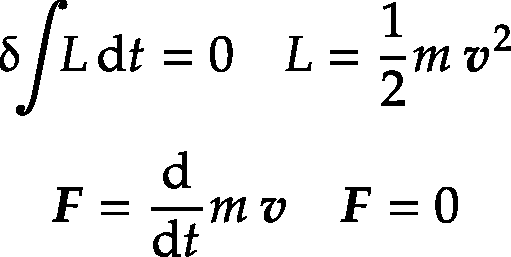
\includegraphics[width=\linewidth]{eg_languages.png}
\\[\jot]{\color{green}%
Example of two different languages expressing the same physical phenomenon%
}
\end{wrapfigure}
Welcome back! The only thing about physics that I need to say here is that physics can be expressed and written from wildly different points of view, using wildly different principles. Let's call these \enquote{different physics languages} (don't take this expression too literally, or as one in common use; I'm just using it for the present discussion). One may approach a physics phenomenon or problem in terms of \emph{Lagrangeans}, or \emph{Hamiltonians}, or \emph{fibre bundles}, or \emph{categories}, or \emph{action principles}, or many other points of view. These languages are not completely separated; we know how to translate among them. In \enquote{doing} physics, one may jump among languages, because some ideas may be easier to express, or some results easier to find, in one language than another. No matter which physics language you choose, the results and the concrete applications are still the same. The choice is to a great extent subjective, based on your aesthetic tastes. You see that in \enquote{doing} physics you can express your personality and put your own artistic touch; this is why it's such a cool subject (and other subjects are like this too).

In these notes I'm choosing one particular language: the one that for me is the most easily \emph{visualizable}; because I believe that visualization can be beneficial in learning new things. Or maybe I'm choosing it just because I like it best. I encourage you to explore how the physics you've learned is expressed in other physics languages; maybe you'll like another physics language better.

The language we'll be using might be called \enquote{field theory}. Roughly speaking it takes as starting point the ideas of space and time, or better spacetime, in which there are different kinds of \enquote{stuff}. It expresses the regularity and patterns that we observe in physical phenomena as \enquote{budgets} about the different kinds of stuff, and of relations between these kinds. Please don't take the description just given too literally; it's just meant to give you a very vague idea of the field-theoretical viewpoint.

\medskip

\begin{wrapfigure}{r}{0.3\linewidth}\scriptsize% with wrapfigure
{\color{green}\enquote{\emph{this grand book, the universe, which stands continually open to our gaze. But the book cannot be understood unless one first learns to comprehend the language and read the
letters in which it is composed. It is written in the language of
mathematics}}\sourceatright{\cites{galilei1623}}}
\end{wrapfigure}
It goes without saying that all these \enquote{physics languages} are to a great extent mathematical.

One reason is that numbers allow us to convey information in a concise and precise way. Imagine you have to tell someone, who doesn't know Bergen, where in Bergen you are right now, to within 10\,m. You can do that with a description, \enquote{\textellipsis\ and there's a building called so-and-so which looks like so-and-so\textellipsis}, which would be lengthy and tricky. Or you can just give two numbers: latitude and longitude:
\begin{equation*}
  \num{60.36940},\ \num{5.3518} \ .
\end{equation*}
And in these two numbers all digits are important; for instance, the latitude is not \ensuremath{60.369\,4\bm{7}}.

\begin{wrapfigure}{r}{0.3\linewidth}\scriptsize% with wrapfigure
{\color{green}\enquote{\emph{There is nothing that can be said by mathematical symbols and relations which cannot also be said by words. The converse, however, is false. Much that can be and is said by words cannot successfully be put into equations, because it is nonsense.}}\sourceatright{\cites{truesdell1966}}}
\end{wrapfigure}
But the most important reason is that mathematics allows us to describe and follow the patters and variety of physical phenomena in a greatly concise and precise way. And to develop their relationships in a rigorous way. All our present technology would have been impossible to discover, and would be impossible to realize, without the mathematical language of physics.

I invite you again to read what many good texts say about the relationship between physics and mathematics. No point repeating here what has been said better elsewhere.

\subsection{Quantities, primitive and derived}
\label{sec:primitives}

One topic, however, must be briefly discussed because it's important in understanding the notes that follow. It's the distinction between \emph{primitive} and \emph{derived} quantities.

I shall assume that you already know what a \emph{physical quantity} is. Examples are: position, duration, velocity, pressure, energy, temperature.

A \emph{derived quantity} is one that is defined in terms of other quantities. For example, velocity $\bm{v}$ (more precisely: average velocity) is defined as the ratio between a distance $\bm{d}$ (a vector) and a time duration $\bm{t}$:
\begin{equation*}
  \bm{v} \defd \frac{\bm{d}}{t}
\end{equation*}
where the symbol \enquote{$\defd$} means \enquote{is defined as} or \enquote{is defined by}. This means that in principle we could avoid using the word \enquote{velocity} and the symbol \enquote{$\bm{v}$} altogether, and instead always speak about distance and duration, using their symbols. It would be extremely inconvenient, but it could be done. The definition of a derived quantity often tells us how that quantity can be measured.

A derived quantity is defined in terms of other quantities, and these may in turn be derived quantities, that is, defined in terms of still other quantities, and so on. But at some point this chain of definitions must come to an end, otherwise we would go around in circles.

A \emph{primitive quantity} is one that we do not define in terms of other quantities. Primitive quantities are the building blocks from which we define all others. That they are not defined in terms of others doesn't mean that we cannot try to explain them. But such explanations must be taken as informal and heuristic. Primitive quantities are often explained through metaphors and by appealing to intuition. You must always be wary of such explanations, because they may fail you spectacularly in some situations.

Often we have a choice about which quantities should be primitive and which should be derived. For instance, \emph{energy} can be defined, in a somewhat complicated way, in terms of quantities like \emph{work} and \emph{heat}, which would then need to be taken as primitive. Or we can take \emph{energy} as primitive, and define \emph{work} and \emph{heat} in terms of it; this second choice turns out to be more convenient to develop the physical theory. It often happens that a quantity is very convenient to build a theory if used as primitive, but difficult to understand intuitively; and vice versa that a quantity is very intuitive, but leads to a complicated theory.

Among quantities which we'll take as primitive are \emph{time}, \emph{space}, \emph{energy}, \emph{matter}, \emph{momentum}, and several others.




% ** 7
% *** Experimental characteristics of time measurement:
% **** time is not universal; for many purposes we must use a time _coordinate_ (maybe a simple spacetime diagram)
% **** GPS?
% **** luckily for many phenomena on Earth the difference is small
% *** Coordinate systems; vectors
% *** Experimental characteristic of quantities:
% **** quantities are "primitives"
% **** dependence on coordinate system

\newpage

\section{Time, space, \enquote{stuff}}
\label{sec:time_space_stuff}

\subsection{Time}
\label{sec:time}



\begin{wrapfigure}{r}{0.3\linewidth}\scriptsize% with wrapfigure
  {\color{green}\enquote{\emph{%
        In 1976, the International Astronomical Union introduced relativistic concepts of time and the transformations between various time scales and reference systems. \textelp{} Now \textelp{} it is necessary to base all astrometry, reference systems, ephemerides, and observational reduction procedures on consistent relativistic grounds. This means that relativity must be accepted in its entirety, and that concepts, as well as practical problems, must be approached from a relativistic point of view.}}\sourceatright{\cites{kovalevskyetal2004}}}
\end{wrapfigure}
\emph{Time} is a primitive quantity. We understand the notion of time intuitively, even if it's difficult to explain (that's why it's taken as primitive). In 1905, with the theory of relativity, part of our everyday intuition about this notion was seriously shaken. For many years afterwards our old intuition could still be used in practice and in applications. But the new, correct intuition is becoming more and more important in everyday life and technologies. For example, GPS navigation, which we use everyday from leisure activities such as hiking or sightseeing to more critical ones such as aeroplane landing, critically depend on the correct notion and intuition of time. Let's see how our traditional intuition goes astray with a concrete experiment.

Here's Alice, Bob, and Charlie. They have extremely precise clocks built in exactly the same way. They stay very close to one another and synchronize their clocks. Still keeping close, they go around, maybe on an aeroplane or space ship, and all the time they check their clocks. They notice that their clocks stay perfectly synchronized all the time, no matter where they go and what they do.

At some point they separate, each one going around independently. One of them might stay in place, another might take a helicopter, and another might go for a trip on Mars and back.

Alice and Bob at some point meet again, and compare their clocks. They see that their clocks aren't synchronized anymore; the difference could be as small as microseconds, or as large as years. In fact, if this time discrepancy is large, they would notice that they themselves have aged differently; so time discrepancy doesn't affect the clocks only. Let's say for concreteness that Alice's clock is ahead of Bob's, or equivalently that Bob's is behind Alice's. Note the following aspects:

First, neither Alice or Bob can say \enquote{my clock was wrong}: neither has noticed anything strange about the \enquote{passage of time}.

Second, they might wonder what's the time on Charlie's clock. But Charlie is at some distance away. They could decide to contact Charlie via radio, say, and ask \enquote{what shows your clock right \emph{now}?}. But they would notice that there's a delay, even if extremely small, in the radio transmission; so it's unclear to what time would Charlie's answer apply. If we say \enquote{let's account for the radio-signal speed}, we see that there's a logical problem: speed is distance divided by time, and here we have a problem in exactly determining what's the \enquote{correct} time! So we would be reasoning in circles. Besides, even neglecting these difficulties, Charlie's answer could reveal a time that completely different from Alice's and from Bob's -- it could be years ahead or behind both of theirs!

Third, if they now stay together, they will see that their clocks remain exactly synchronized, besides the discrepancy they noticed when they met. This discrepancy doesn't increase or decrease. They may even retrace together Alice's and Bob's previous trips; their clocks still remain synchronized.

The experience just described will occur again any time two or more of them meet. There could be a hundred observers like Alice, Bob, Charlie, initially at the same place and synchronized. Whenever two or more of them meet after having been separated, they will notice discrepancies in their clocks. But their clocks will have exactly the same time lapses as long as they stay together.

Consider for a moment an imaginary world in which these experiments had given a different kind of result. According to Newtonian mechanics, whenever two or more initially synchronized observers like Alice, Bob, Charlie had met, their clocks would have always shown exactly the same time. If one year, 23 days, 8 hours, 9 minutes, and \num{3.04539928324099266302} seconds have passed for you since you last met Alice, you'd see that exactly the same amount of time has passed for her when you two meet again. If you think about it, in this case it would have beeen somewhat natural to think \enquote{right now, the clocks of far-away Alice, Bob, Charlie must show the same time as mine} (even though you have no real experimental way of confirming that).

But that's an imaginary world. In our world is the more complicated situation described initially that holds. Only one conclusion can be drawn from these experimental results: \textbf{Time is not some sort of universal quantity. It is, so to speak, \enquote{local} to a person or clock, or to a group of persons or clocks that stick together.} This also means that \emph{it doesn't make sense} to ask questions like \enquote{what can be the time for far-away Charlie, right now?}. % \emph{Now} only applies to you, or to anything that is in your immediate vicinity.

\smallskip

The time measured by a specific observer is called the \emph{proper time} of that observer. Luckily we know more about how the proper times of separated observers can differ when they meet again. It turns out -- according to our current understanding -- that the time differences depend, roughly speaking, on how fast the observers are moving with respect to one another and to matter around the universe, and on how much energy is contained in the regions they travel. The general theory of relativity gives us the equations determining any such proper-time differences.

\begin{wrapfigure}{r}{0.3\linewidth}\scriptsize% with wrapfigure
{\color{green}\enquote{\emph{%
The plot for Cesium \textelp{} characterizes the best orbiting clocks in the GPS system. What this means is that after initializing a Cesium clock, and leaving it alone for a day, it should be correct to within \textelp{} \num{4}~nanoseconds. Relativistic effects are huge compared to this.}}\sourceatright{\cites{ashby2003}}}
\end{wrapfigure}
The situation depicted in the experiments above is real. It can be measured, for example, comparing initially synchronized clocks that have been put in aeroplanes flying in different directions. Most importantly, it affects everyday relevant technologies such as the Global Positioning System. Formulae from general relativity appear in your phone's GPS software; see for instance \sect~20.3.3.3.3 of the Interface Control Document \texttt{IS-GPS-200} at \url{https://www.gps.gov/technical/icwg/}. It must also be taken into account in the establishment and synchronization of time in our everyday equipments:
%\autocites[]{icwg1983_r2022}
\begin{quote}\footnotesize
International Atomic Time (TAI) is based on more than 250
atomic clocks
distributed worldwide that provide its stability,
whereas a small number of primary frequency standards
provide its accuracy. Universal Coordinated Time,
which is the basis of all legal time scales, is derived from TAI.
To allow the construction of TAI and the general dissemination
of time, clocks separated by thousands of kilometres must
be compared and synchronized. \textelp{}
The achieved performances of atomic clocks and time
transfer techniques imply that the definition of time scales
and the clock comparison procedures must be considered
within the framework of general relativity.
\sourceatright{(\cites{petitetal2005})}
%\mbox{}\hfill (\cites{petitetal2005})
\end{quote}
% \begin{figure}[h!]\scriptsize\centering% with wrapfigure
% 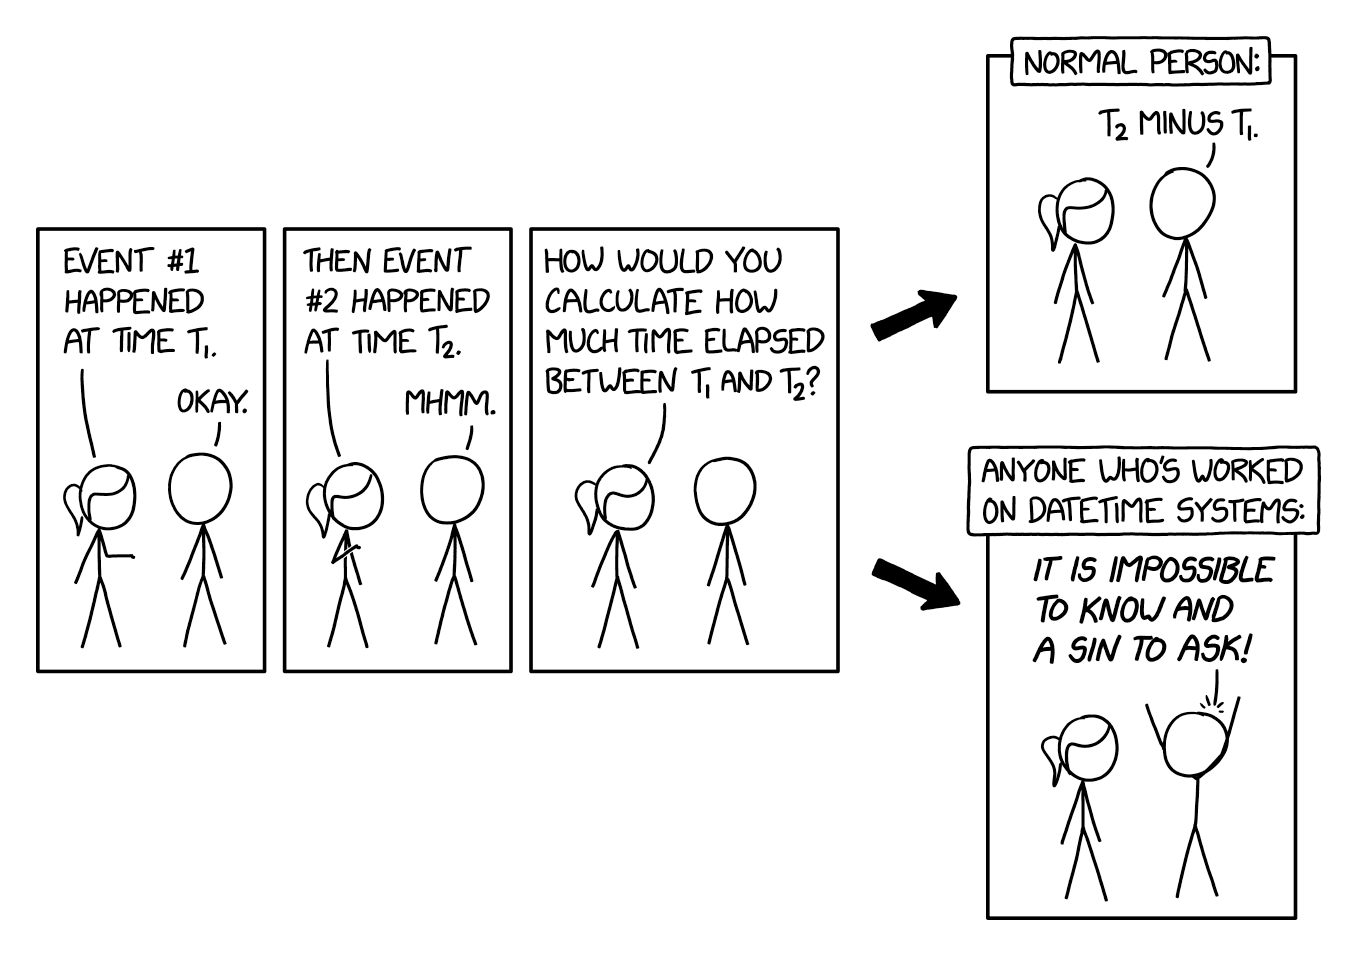
\includegraphics[width=0.75\linewidth]{datetime_2x.png}
% \\%
% \url{https://xkcd.com/2867}
% \end{figure}


\smallskip

Together with the notion of time, also the notion of space loses some of its traditional intuition; but we shall not delve further into these topics. Keep simply in mind that phenomena happen in \emph{spacetime}, and that there's no way to attribute a universal time, nor a universal position in space, to a physical event. There is one absolute: whoever locally measures the speed of light, will find the value $c\defd \qty{299792458}{m/s}$. This value is exact by definition, and serves as a way to define a local notion of space.

In most everyday situations for us, who live on or nearby Earth and move at speeds much smaller than $c$ with respect to one another, the discrepancies between our proper times are so small that cannot be
measured with ordinary clocks or with our internal clocks. Consider a
person walking \qty{10}{m} away from you and then immediately walking back
to you, at \qty{1}{m/s}. The time elapsed for you will be \qty{20}{s}, but for that person
\begin{wrapfigure}{r}{0.3\linewidth}\scriptsize\centering% with wrapfigure
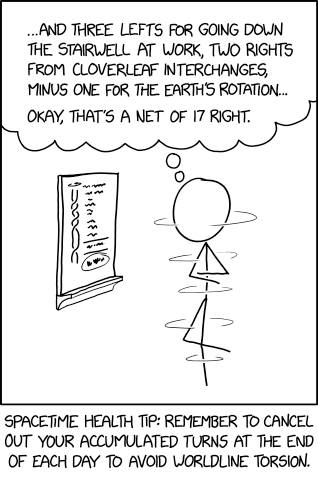
\includegraphics[width=\linewidth]{net_rotations.png}
\\%
\url{https://xkcd.com/2882}
\end{wrapfigure}
will be \qty{19.999999999999999889}{s}, a difference of \qty{e-16}{s}, which is the error of an atomic clock. %%***add ref
If human beings still exist in some decades or centuries, with space travel they will probably have to deal more and more with proper-time discrepancies also in everyday life.

For the most part of the rest of these notes, we won't need to deal with differences in proper time. But I recommend that you keep present how time really works, and that these small time discrepancies exist and occur all the time along your \emph{worldline}.

% In Bergen, a distance of 10\,m corresponds to a difference of 0.000\,1\,° in latitude or longitude


\subsection{Coordinate systems}
\label{sec:coords}

It is necessary to have a way to distinguish physical events and processes and locate them in spacetime. This is done through a \emph{coordinate system}. A coordinate system assigns four numerical labels to every point in spacetime. Often these labels have some kind of physical meaning, such as the proper time elapsed for a specific clock, or the distance from some event, but they don't need to.

A coordinate system also solves the problems coming from proper-time discrepancies. We can assign to every physical event a \emph{coordinate time}, which is the same for all observers and decided by agreement. Coordinate time doesn't have a strict physical meaning, and will generally be different from the proper times registered by different observers. It can nevertheless be used for \enquote{doing physics}, and it is the time we shall most often use in our equations. A coordinate time commonly used for Earth-physics purposes is \href{https://www.nist.gov/pml/time-and-frequency-division/time-realization/utcnist-time-scale-0}{Universal Coordinated Time (UTC)}\footnote{\url{https://www.nist.gov/pml/time-and-frequency-division/time-realization/utcnist-time-scale-0}}. The clock on your phone, and on devices that get synchronized via internet, shows UTC -- not your proper time. An observer on Earth at \qty{0}{m} over sea level, and not moving, measures a proper time exactly equal to UTC (besides small variation coming from the movements of Solar System bodies). Observers at other altitudes or moving with respect to Earth's surface notice that their proper times are slightly different from UTC.

It is always important to specify how the coordinate system you're using is defined. This specification is of course silently understood among people who have decided on a coordinate system beforehand. We shall often denotes the four coordinates of a coordinate system by
\begin{equation*}
  (t, x, y, z)
\end{equation*}
where $t$ is a coordinate time, usually UTC, and $(x,y,r)$ determine a spatial position. This triplet of spatial coordinates is often denoted by the vector $\yr$:
\begin{equation*}
  \yr \defd (x,y,z) \ .
\end{equation*}




% 
% ** 8
% *** Structure of physical laws:
% **** fundamental
% **** constitutive
% **** boundary & initial conditions
% *** Conservation and balance laws
% *** Seven wonders of the world: geometric meaning; maths translation
% *** Why different phenomena and how to make predictions: Constitutive equations
% *** Conservation of amount of matter
% **** examples
% 
% ** 9
% *** Energy: characteristics
% **** coordinate-dependent
% **** mass is energy, energy is mass
% **** matter: necessity of separation between "bulk" (mass) and small changes (energies); examples
% *** Balance of energy
% **** energy is only balanced; cosmology
% 
% ** 10
% *** Momentum: characteristics
% **** coordinate-dependent
% **** momentum is energy flow, and vice versa
% **** matter: necessity of separation between "bulk" (momentum) and small changes (heat); examples
% *** Balance of momentum
% *** Force is momentum current; examples (diSessa)
% 
% ** 11
% *** Rotational momentum
% *** Balance of rotational momentum
% *** Interlude: Conservation of charge and of magnetic flux
% *** Balance of entropy; "second law"
% 
% ** 12
% *** _Special constitutive equations of Newtonian mechanics:_
% *** Momentum ∝ matter flux; difference in relativity
% *** Forms of energy beside the "bulk"
% **** kinetic
% **** potential gravitational
% **** internal; several types (including chemical, elastic, etc)
% *** TODO Check work and heat
% 
% ** 13
% *** _Example systems and problems_
% 
% ** 14
% *** Temperature
% *** Entropy flux is (energy flux)/(temperature)
% 
% ** 15
% *** Constitutive equations for internal energy: ideal gas (with dV/dt term)
% *** _Example systems and problems_
% 
% ** 16
% *** Other examples: GPS?




\iffalse
\begin{wrapfigure}{r}{0.3\linewidth}\scriptsize% with wrapfigure
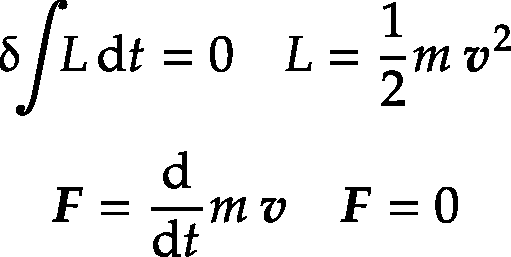
\includegraphics[width=\linewidth]{eg_languages.png}
\\[\jot]%
{\color{green}\enquote{\emph{%
}}\sourceatright{\cites{}}}
\end{wrapfigure}
\fi




\newpage

\section{The Seven Wonders of the world}
\label{sec:seven_wonders}


% https://education.nationalgeographic.org/resource/seven-wonders-ancient-worl

\newpage

\section{Thermodynamics}
\label{sec:thermodynamics}

\subsection{Notes on \enquote{quasi-static} processes}
\label{sec:quasistatic}

In general, none of the statements "reversible${}\Rightarrow{}$quasi-static" or "quasi-static${}\Rightarrow{}$reversible"
is true.

A counterexample to the second implication are systems with internal state variables, which cannot be made non-dissipative, no matter how slowed-down they are. See the discussion and mathematical analysis in Astarita \sect~2.5.


A counterexample to the first implication is a system of spins in a crystal lattice. It is possible to \emph{reversibly} bring the system form an equilibrium state to another with opposite temperature by reversing the external magnetic field \emph{as fast as possible} – and therefore \emph{not} through a quasi-static process. In fact it is key here that the process be \emph{not}-quasi-static, but as fast as possible, because a slow change of the external magnetic field would lead to an irreversible process with dissipation. For more details see the discussion in Buchdahl, Lecture~20.

The point is that for some systems a \emph{fast} change can actually prevent the onset of dissipative phenomena, and so the process needs to be fast if we want it to be reversible. Adiabatic processes often also need to be fast (as a curious historical fact, Truesdell \amp\ Bharatha, Preface p.~xii, remark that \enquote{In introducing what we today call an `adiabatic process', Laplace called it `a sudden compression', in which he was followed by Carnot}).

In fact, clearly non-quasi-static phenomena such as \emph{explosions} can in some circumstances be described by \emph{reversible} processes! This is possible if the explosion involves many shock waves, as explained by Oppenheim, chap.~1 p.~63:
\begin{quote}
  If there is more than one shock, the losses in available energy are diminished, so that in the limit, with an infinite number of shocks, they become negligible, and the process acquires the character of a thermodynamically optimal, i.e., reversible, change of state. The study of explosion processes reveals that, indeed, they are associated not with one but with a multitude of shocks.
\end{quote}
For explosions see also the mathematical analysis by Dunwoody: \emph{Explosion and implosion in a mixture of chemically reacting ideal gases}, where again reversible-process equations are used.

A caveat about reversible and quasi-static associations is given by Ericksen (\sect~1.2):
\begin{quote}
  Some tend to associate nearly reversible processes with those taking place very slowly – the "quasi-static" processes. This probably stems, at least in part, from experience with classical theories of heat conduction, viscosity, and so on. However, a ball made of silly putty behaves almost reversibly when bounced rapidly and various other high polymers have similar predilections. So, it seems prudent to be open-minded in considering what may be reversible processes for particular systems.
\end{quote}
He later discusses (\sect~3.1) the case of bars subjected to dead loads, for which we can have reversible processes under sudden jumps in elongation. He concludes (p.~46) that \enquote{the sudden jump provides an example of a process that is reversible but not reasonably considered to be quasi-static}.

\medskip

But there's an important question that underlies our discussion: what do we actually mean by \enquote{quasi-static}? We need to specify a time scale, otherwise the term is undefined. For example, a geological process (say, tectonic motion) can be considered as quasi-static – or even completely static – on time scales of minutes or days; but it is not quasi-static on time scales of millions of years.

Whether a process is reversible or not, within any tolerance needed, is an experimental question. We can measure any relevant quantities, say pressure $p$ and exchanged heat $q$, under the process, and compare them with those, $p^*$ and $q^*$, determined by the equations for a reversible process. We may find for example that at all times
$$\biggl\lvert\frac{p - p^*}{p^*}\biggr\rvert < 0.001 \ ,
\quad
\biggl\lvert\frac{q - q^*}{q^*}\biggr\rvert < 0.001
$$
and conclude that the process is reversible, if relative discrepancies of $0.1\%$ or less are negligible in our concrete application.

But suppose that someone tells us \enquote{if you want the process to be reversible, you must make sure that it is quasi-static}. Alright, but how much is \enquote{quasi-static}? is it OK if the piston moves with a speed of 1~cm/s? or is that too much? How about 1~mm/s? – In fact we may find that for some kind of fluid 1~cm/s is absolutely acceptable for the process to be reversible, whereas for another kind of fluid that speed would lead (at the same temperature) to an irreversible process.

You see how this imprecise situation can lead to circular definitions: "if the process is irreversible, then it means it isn't quasi-static" – but then we are actually \emph{defining} "quasi-static" in terms of "reversible"! Any statement of the kind "reversible${}\Rightarrow{}$quasi-static" or "quasi-static${}\Rightarrow{}$reversible" then becomes not a matter of experimental verification, but of pure \emph{semantics}. At this point we can simply get rid of "quasi-static" terminology since it doesn't bring any new physics to the table. This circularity is admitted for example by Callen in discussing irreversible gas expansion (Problem 4.2-3 p.~99):

\begin{quote}
  The fact that $dS > 0$ whereas $dQ = 0$ is inconsistent with the presumptive applicability of the relation $dQ = T\,dS$ to all quasi-static processes. We define (by somewhat circular logic!) the continuous free expansion process as being "essentially irreversible" and \emph{non-quasi-static}.
\end{quote}

A similar criticism can be read in Astarita, \sect~2.9, p. 62, where he also provides a mathematical quantification of quasi-static, similar to the one given above for reversibility:

\begin{quote}
  Often this point is circumvented by bringing in another difficult concept,
  that of a quasi-static transformation, which proceeds "through a sequence of
  equilibrium states." Quasi-static is an impressive word, but the only meaning
  which can be attached to it is the less impressive word "slow" – and how can
  one speak of slowness without implying the concept of time? How slow is slow
  enough? If one chooses to develop a thermodynamic theory (rather than a
  thermostatic one), the answer is easy. For instance, in the case of a system where
  the state is $V, T, \dot{V}$ [the latter is the rate of change of $V$], one needs to assume that [the non-equilibrium pressure] $p(V,T,\dot{V})$ is a Taylor-series expandable
  at $\dot{V} = 0$ to obtain [that
  $$
  p = p^* + \frac{\partial p}{\partial \dot{V}}\biggl\lvert_{\dot{V}=0}\dot{V} + \mathrm{O}(\dot{V}^2) \ ,
  $$
  where $p^* = p(V,T,0)$ is the pressure at equilibrium]. One then reaches the conclusion that if the
  condition
  $$\dot{V} \ll \frac{p^*}{\partial p/\partial \dot{V}\lvert_{\dot{V}=0}}
  $$
  is satisfied, then indeed the difference between $p$ and $p^*$ is negligibly small as compared to $p^*$, and thus the process can be regarded as a quasi-static one.
\end{quote}

Criticisms against the fuzzy notion of "quasi-static" have appeared in many other works. Truesdell \amp\ Bharatha (Preface p.~xii), make the historical remark that "the 'quasi-static process' was barely mentioned for the first time in 1853 and was altogether foreign to the early work [in thermodynamics]". See also the mathematical analysis by Serrin: \emph{On the elementary thermodynamics of quasi-static systems and other remarks}.

\medskip

I also want to point out that "quasi-static" in some works has specific meanings somewhat unrelated to the discussion above. For example that the rate of increase of the total kinetic energy $K$ of the system is negligible, so that the law of energy balance, which in its full generality is
$$ \frac{\mathrm{d}(U+K)}{\mathrm{d}t}  = Q + W$$
(that is, the rate of increase of internal energy $U$ and kinetic energy is equal to the heat rate $Q$ and work rate $W$ provided to the system) can be approximated by
$$ \frac{\mathrm{d}U}{\mathrm{d}t}  = Q + W \ .$$
Or that similar inertial terms in the motion of the system are negligible. See for example the book by Day, chap.~2.

But note that such definitions of "quasi-static" have, again, \emph{no} a-priori relation with reversibility.

\medskip

Finally, the equation $\mathrm{d}S = Q/T$ is only valid for a process that is:
\begin{itemize}
\item reversible (by definition),
\item closed (no exchange of mass),
\item with a homogeneous surface temperature,
\item without bulk heating (such as instead happens in a microwave oven).
\end{itemize}
Under the last three conditions we have in general that $\mathrm{d}S \ge Q/T$; when the equality sign is satisfied, then the process is \emph{defined} as reversible. See Astarita, \sect~1.5, or Müller \amp\ Müller, for the different forms of the second law under different circumstances. This equation may be valid in quasi-static and non-quasi-static processes, as explained above.

% ### References ###

% I recommend you do your own reading and eventually reach your own conclusions about your question.

% * Astarita: [*Thermodynamics: An Advanced Textbook for Chemical Engineers*](https://doi.org/10.1007/978-1-4899-0771-4).

% * Buchdahl: [*Twenty Lectures on Thermodynamics*](https://doi.org/10.1016/C2013-0-02649-7).

% * Callen: [*Thermodynamics: an introduction to the physical theories of equilibrium thermostatics and irreversible thermodynamics*](https://books.google.com/books/about/Thermodynamics_an_Introduction_to_the_Ph.html?id=V_1LzQEACAAJ) (Wiley 1960).

% * Day: [*Heat Conduction Within Linear Thermoelasticity*](https://doi.org/10.1007/978-1-4613-9555-3).

% * Dunwoody: [*Explosion and implosion in a mixture of chemically reacting ideal gases*](https://doi.org/10.1007/BF02133864).

% * Ericksen: [*Introduction to the Thermodynamics of Solids*](http://d-nb.info/95351451X/04) (Springer 1998).

% * Müller, Müller: [*Fundamentals of Thermodynamics and Applications: With Historical Annotations and Many Citations from Avogadro to Zermelo*](https://doi.org/10.1007/978-3-540-74648-5). This is book with a large amount of concrete applications (from jet engines to pneumatic compressors) of thermodynamics and thermostatics.

% * Oppenheim: [*Introduction to Gasdynamics of Explosions*](https://doi.org/10.1007/978-3-7091-4364-3).

% * Serrin: *On the elementary thermodynamics of quasi-static systems and other remarks*, in Brock (ed.): [*Thermoelastic Problems and the Thermodynamics of Continua*](https://books.google.com/books/about/Thermoelastic_Problems_and_the_Thermodyn.html?id=I_1QAAAAMAAJ) (American Society of Mechanical Engineers, 1995).

% * Truesdell, Bharatha: [*The Concepts and Logic of Classical Thermodynamics as a Theory of Heat Engines*](https://doi.org/10.1007/978-3-642-81077-0).




%%%% examples use empheq
%   \begin{empheq}[left={\mathllap{\begin{aligned}    \de\yF_{\yc}/\de\yp&=0\text{:} \\
%         \de\yF_{\yc}/\de\ym&=0\text{:}\\ \de\yF_{\yc}/\de\yl&=0\text{:}\end{aligned}}\qquad}\empheqlbrace]{align}
%     \label{eq:con_p}
% %    \de\yF_{\yc}/\de\yp &\equiv
%     -\ln\yp + \ln\yq + \yl\yM + \ym\yu &=0,\\
%     \label{eq:con_u}
% %    \de\yF_{\yc}/\de\ym &\equiv
%     \yu\yp-1 &=0,\\
%     \label{eq:con_l}
%     %\de\yF_{\yc}/\de\yl &\equiv
%     \yM\yp-\yc &=0.
%   \end{empheq}
%%%%
% \begin{empheq}[box=\widefbox]{equation}
%   \label{eq:maxent_question}
%   \p\bigl[\yE{N+1}{k} \bigcond \tsum\yo\yf{N}\in\yA, \yM\bigr] = \mathord{?}
% \end{empheq}


%%\setlength{\intextsep}{0ex}% with wrapfigure
%%\setlength{\columnsep}{0ex}% with wrapfigure
%\begin{figure}[p!]% with figure
%\begin{wrapfigure}{r}{0.4\linewidth} % with wrapfigure
%  \centering\includegraphics[trim={12ex 0 18ex 0},clip,width=\linewidth]{maxent_saddle.png}\\
%\caption{caption}\label{fig:comparison_a5}
%\end{figure}% exp_family_maxent.nb


%%%%%%%%%%%%%%%%%%%%%%%%%%%%%%%%%%%%%%%%%%%%%%%%%%%%%%%%%%%%%%%%%%%%%%%%%%%%
%%% Acknowledgements
%%%%%%%%%%%%%%%%%%%%%%%%%%%%%%%%%%%%%%%%%%%%%%%%%%%%%%%%%%%%%%%%%%%%%%%%%%%% 
\iffalse
\begin{acknowledgements}
  \ldots to Mari \amp\ Miri for continuous encouragement and affection, and
  to Buster Keaton and Saitama for filling life with awe and inspiration.
  To the developers and maintainers of \LaTeX, Emacs, AUC\TeX, Open Science
  Framework, R, Python, Inkscape, Sci-Hub for making a free and impartial
  scientific exchange possible.
  % Our work was supported by the Trond Mohn Research Foundation, grant number BFS2018TMT07
%\rotatebox{15}{P}\rotatebox{5}{I}\rotatebox{-10}{P}\rotatebox{10}{\reflectbox{P}}\rotatebox{-5}{O}.
%\sourceatright{\autanet}
\mbox{}\hfill\autanet
\end{acknowledgements}
\fi

%%%%%%%%%%%%%%%%%%%%%%%%%%%%%%%%%%%%%%%%%%%%%%%%%%%%%%%%%%%%%%%%%%%%%%%%%%%%
%%% Appendices
%%%%%%%%%%%%%%%%%%%%%%%%%%%%%%%%%%%%%%%%%%%%%%%%%%%%%%%%%%%%%%%%%%%%%%%%%%%% 
%\clearpage
% %\renewcommand*{\appendixpagename}{Appendix}
% %\renewcommand*{\appendixname}{Appendix}
% %\appendixpage
% \appendix

%%%%%%%%%%%%%%%%%%%%%%%%%%%%%%%%%%%%%%%%%%%%%%%%%%%%%%%%%%%%%%%%%%%%%%%%%%%%
%%% Bibliography
%%%%%%%%%%%%%%%%%%%%%%%%%%%%%%%%%%%%%%%%%%%%%%%%%%%%%%%%%%%%%%%%%%%%%%%%%%%% 
\newpage
\renewcommand*{\finalnamedelim}{\addcomma\space}
\defbibnote{prenote}{{\footnotesize (\enquote{de $X$} is listed under D,
    \enquote{van $X$} under V, and so on, regardless of national
    conventions.)\par}}
% \defbibnote{postnote}{\par\medskip\noindent{\footnotesize% Note:
%     \arxivp \mparcp \philscip \biorxivp}}

\printbibliography[prenote=prenote%,postnote=postnote
]

\end{document}

%%%%%%%%%%%%%%%%%%%%%%%%%%%%%%%%%%%%%%%%%%%%%%%%%%%%%%%%%%%%%%%%%%%%%%%%%%%%
%%% Cut text (won't be compiled)
%%%%%%%%%%%%%%%%%%%%%%%%%%%%%%%%%%%%%%%%%%%%%%%%%%%%%%%%%%%%%%%%%%%%%%%%%%%% 

The theory of relativity -- by which we mean _general_ relativity in these notes -- is now more than 100 years old. And yet, its equations are today necessary for many common technologies, like nuclear reactors and the [Global Positioning System](https://www.gps.gov); and some of the phenomena it predicts, like [black holes](https://spaceplace.nasa.gov/black-holes) and [gravitational waves](https://spaceplace.nasa.gov/gravitational-waves), have been experimentally detected only more than 100 years after its birth.

Relativity theory is based on ideas and notions that are in some respects different from classical Newtonian physics. Some of these ideas are common knowledge today; for example the fact that mass is a form of energy, and that gravitational force comes from the curvature of spacetime.

Seeing the practical importance of relativity in today's technology, its presence in common knowledge, and its age, it is surprising that 1st-year undergraduate physics courses still teach old and not-quite-correct ideas and notions.

Some teachers say "it would be too difficult for students to understand relativity ideas, because they are too familiar with the old ones. This is why we need to teach the old and slightly incorrect ideas first, and correct them later". I think that this kind of reasoning is scientifically unacceptable and leads to a vicious circle. Students are unfamiliar with the new scientific ideas only because they were raised by a generation who was taught the old ideas. New ideas become familiar if we have a couple of generations that learn them early. This is quite obvious if you think that ideas such as energy and electromagnetic fields are very familiar today, but were absolutely _un_familiar centuries ago. If we were always to teach what's familiar, then we would still be teaching about the "elements" _air_, _earth_, _water_, _fire_, and that the Sun revolves around the Earth.

It is moreover not fully true that the new ideas are unfamiliar to students; quite the opposite. Students know, for example, about the equivalence between mass and energy. When the students see how these notions are presented as very distinct things in 1st-year physics, they get slightly confused. Indeed many students end up asking very intelligent questions, such as "should the mass of the body be included in its internal energy?".

I therefore think that it is due time to replace the old ideas and notions still taught in 1st-year undergraduate physics with the new ones. Maybe one or two generations of students will face some discomfort in this transition, but the subsequent generations will enjoy the benefits. Instead of wasting time learning partly incorrect ideas and correcting them later (as if our lifespans were infinite), students should learn correct ideas at the very start, in order to directly use or deepen them later.

But the discomfort of this transition is not so great, after all. Many important notions from relativistic physics can be introduced in classical physics in a simple and natural way. Most maths and symbols remain practically the same, but we can attach to them more correct meanings.

These lecture notes are an attempt at making such a transition.


%%% Local Variables: 
%%% mode: LaTeX
%%% TeX-PDF-mode: t
%%% TeX-master: t
%%% End: 
